\pdfoutput=1
\documentclass[11pt]{article}

\usepackage[T1]{fontenc}
\usepackage{lmodern}
\usepackage[margin=1in]{geometry}
\usepackage{microtype}
\usepackage{amsmath,amssymb,amsthm,mathtools}
\usepackage{booktabs,array}
\usepackage{needspace,float}
\usepackage{multicol}
\usepackage{xcolor}
\usepackage{tikz}
\usetikzlibrary{arrows.meta,positioning,calc}
\usepackage[hidelinks]{hyperref}

\hypersetup{
  pdftitle={From Chirality to the Standard Model: A Uniqueness and No-Go Theorem for Compact Lie-Algebra Embeddings},
  pdfauthor={Emad Mostaque},
  pdfsubject={A classification of effective compact Lie-algebra pairs with complex-type adjoint complement and nonzero cubic radical, and extremal E6 subgroup chains},
  pdfkeywords={chirality, cubic anomaly, compact Lie algebras, uniqueness theorem, no-go theorem, adjoint complement, homogeneous realization, E8, E6, extremal subgroups, Standard Model, left-right symmetry, charge quantization, three generations}
}

\setlength{\parindent}{1.2em}
\setlength{\parskip}{0pt}
\setlength{\textfloatsep}{16pt plus 4pt minus 4pt}
\setlength{\floatsep}{14pt plus 3pt minus 3pt}
\setlength{\intextsep}{14pt plus 3pt minus 3pt}
\emergencystretch=2em
\allowdisplaybreaks[2]


\newtheorem{theorem}{Theorem}[section]
\newtheorem{lemma}[theorem]{Lemma}
\newtheorem{proposition}[theorem]{Proposition}
\newtheorem{corollary}[theorem]{Corollary}
\theoremstyle{remark}
\newtheorem*{remark}{Remark}

\tikzset{
  repbox/.style={draw=black,rounded corners=1pt,fill=black!3,
    align=center,inner sep=5pt,font=\small},
  chiralbox/.style={draw=black,line width=.85pt,rounded corners=1pt,fill=black!7,
    align=center,inner sep=6pt,font=\small},
  singletbox/.style={draw=black!65,rounded corners=1pt,fill=black!2,
    align=center,inner sep=6pt,font=\small},
  overviewbox/.style={draw=black!70,rounded corners=2pt,fill=black!2,
    text width=.82\textwidth,align=center,inner sep=4pt,font=\small},
  branch/.style={-{Latex[length=1.8mm]},line width=.6pt}
}

\newcommand{\g}{\mathfrak g}
\newcommand{\h}{\mathfrak h}
\newcommand{\q}{\mathfrak q}
\newcommand{\e}{\mathfrak e}
\newcommand{\su}{\mathfrak{su}}
\newcommand{\soalg}{\mathfrak{so}}
\newcommand{\Tr}{\operatorname{Tr}}
\newcommand{\Rad}{\operatorname{Rad}}
\newcommand{\boxt}{\boxtimes}
\newcommand{\Ksm}{G_{\mathrm{SM}}}
\newcommand{\Klr}{G_{\mathrm{LR}}}
\newcommand{\Kps}{G_{\mathrm{PS}}}

\title{From Chirality to the Standard Model\\[0.45em]
\large A Uniqueness and No-Go Theorem for Compact Lie-Algebra Embeddings}
\author{Emad Mostaque}
\date{6 September 2026\\[0.5em]
\small\href{https://github.com/emad-ii/chirality-standard-model}
{\nolinkurl{github.com/emad-ii/chirality-standard-model}}}

\begin{document}

\maketitle

\begin{abstract}
An inclusion of compact Lie algebras supplies its own representation: the
adjoint complement \(\mathfrak q=\mathfrak g/\mathfrak h\). We classify
effective proper inclusions \(\mathfrak h\subsetneq\mathfrak g\) for which
this real module is irreducible of complex type and the cubic trace tensor
of one complex half has nonzero radical. Effectivity means that no nonzero
ideal of \(\mathfrak g\) is contained in \(\mathfrak h\). Up to
isomorphism of Lie-algebra pairs and duality, the unique solution is
\[
 \mathfrak e_8\supset\mathfrak e_6\oplus\mathfrak{su}(3)_M,
 \qquad V=\mathbf{27}\boxtimes\mathbf3,
 \qquad \operatorname{Rad}(c_V)=\mathfrak e_6.
\]
Every other pair in the stated complex-type domain has zero radical. The
proof covers arbitrary rank: toral gradings enumerate the equal-rank cases,
and index arithmetic and highest-weight arguments exclude the lower-rank
cases. The hypotheses also imply a realization as a compact homogeneous
space with closed isotropy subgroup. The commuting \(SU(3)_M\) factor gives three copies of the
\(\mathbf{27}\) on restriction to \(E_6\).

Inside this \(E_6\), a second classification concerns the \(38{,}880\)
triples formed from its three Weyl orbits of maximal proper closed root
subsystems. There are six orbits of triples. Exactly two have an irreducible
\(A_2\) component in their common intersection; these are the two extremal
orbits. In every triple, one pairwise derived group has strictly greatest
dimension. Using that group in the pair-first construction, compatible
representatives of the extremal orbits give
\[
 G_{\mathrm{SM}}\subset G_{\mathrm{LR}}\subset G_{\mathrm{PS}}
 \subset\operatorname{Spin}(10)\subset E_6^{\mathrm{sc}},
 \qquad Y=T_R^3+\frac{B-L}{2},
\]
including their faithful global forms and charge lattices. The full restriction is
\[
 V|_{G_{\mathrm{SM}}}
 \cong3\,\mathcal F_{\mathrm{SM}}
 \oplus3\,(\mathbf5\oplus\overline{\mathbf5})|_{G_{\mathrm{SM}}}
 \oplus6\,\mathbf1.
\]
Here \(\mathcal F_{\mathrm{SM}}\) is one minimal chiral family. The net
chiral class is \(3\chi(\mathcal F_{\mathrm{SM}})\), up to sign; the
other summands are vectorlike or singlets.
\end{abstract}
\clearpage

\section{Introduction}

Matter in the Standard Model is chiral: left- and right-handed fermions
transform differently under the weak interaction. A consistent chiral gauge
theory must also satisfy anomaly cancellation \cite{ParticleDataGroup}.
These requirements constrain the matter representations. Can a mathematical
formulation of them go further, and determine an internal symmetry and its
matter representation together?

An inclusion of compact real Lie algebras
\(\mathfrak h\subsetneq\mathfrak g\) provides a precise algebraic
question. The adjoint action of \(\mathfrak h\) on \(\mathfrak g\)
induces a representation on the quotient,
\[
 \mathfrak q=\mathfrak g/\mathfrak h.
\]
We call this module the \emph{adjoint complement}. It belongs to the
embedding: changing the pair changes the algebra and its representation together. We study
which pairs satisfy a complex-type condition and a condition on the cubic
trace tensor, without first specifying an exceptional group or a matter
multiplet.

\paragraph{The classification problem.}
We consider all effective proper inclusions of finite-dimensional compact
real Lie algebras: no nonzero ideal of \(\mathfrak g\) is contained in
\(\mathfrak h\). The first condition is
\[
 \operatorname{End}_{\mathfrak h}(\mathfrak q)\cong\mathbb C.
\]
It implies that the real module \(\mathfrak q\) is irreducible and has an
invariant complex structure, unique up to sign. Its complexification is
\(V\oplus V^*\), where \(V\) and \(V^*\) are inequivalent irreducible
representations. Thus irreducibility and complex type are
encoded in one condition, rather than imposed separately.

The second condition concerns the cubic trace tensor \(c_V\) on
\(\mathfrak h\). A generator lies in its radical when inserting that
generator makes the cubic vanish, whatever the other two arguments are.
This radical is automatically an ideal, and we require it to be nonzero:
\[
 \operatorname{Rad}(c_V)\ne0.
\]
The test includes all mixed insertions from \(\mathfrak h\). It is
in general stronger than requiring the cubic to vanish only on a separately specified
gauge subalgebra. The ideal on which the cubic vanishes is determined by
the representation itself.

\paragraph{One pair remains.}
Under these conditions, the pair is unique up to isomorphism of Lie-algebra
pairs and duality:
\[
 \mathfrak e_8\supset\mathfrak e_6\oplus\mathfrak{su}(3)_M,
 \qquad V=\mathbf{27}\boxtimes\mathbf3.
\]
Here \(\boxtimes\) denotes the tensor product for the two simple factors.
The cubic radical is \(\mathfrak e_6\); its commuting factor
\(\mathfrak{su}(3)_M\) acts on a three-dimensional multiplicity space.
Restriction to \(E_6\) therefore gives three copies of the \(\mathbf{27}\).
The embedding and the multiplicity are conclusions of the classification.

The theorem is also an exclusion result. Every inequivalent pair satisfying
the standing algebraic hypotheses and the complex-type condition has
zero cubic radical. Proving that the displayed pair works is therefore
only one part of the argument. We must exclude every other equal-rank and
lower-rank possibility, without a rank cutoff.

\paragraph{Where homogeneity enters.}
The hypotheses imply that \(\mathfrak g\) is simple and \(\mathfrak h\)
is semisimple. They therefore integrate to a compact group \(G\) with a
connected closed subgroup \(H\); the tangent space of \(G/H\) at the
base point is precisely \(\mathfrak g/\mathfrak h\). Homogeneity is the
geometric realization of the algebraic pair, not an additional assumption
about physical spacetime. Section~2 proves this passage. The substantive
restriction is that the representation is the entire adjoint complement
and is irreducible of complex type.

\paragraph{Relation to earlier constructions.}
Ordinary \(SU(5)\), \(\operatorname{Spin}(10)\), and \(E_6\) unification
organizes a family in \(\mathbf{10}\oplus\overline{\mathbf5}\),
\(\mathbf{16}\), or \(\mathbf{27}\), but does not by itself fix how many
times it is repeated \cite{GeorgiGlashow,FritzschMinkowski,GurseyRamondSikivie}.
Homogeneous representations have also been used in coset-space dimensional
reduction and exceptional family unification
\cite{ForgacsManton,MantonFermions,ChaplineSlansky,ChaplineGrossman,
DouzasEtAl,KugoYanagida,ItohKugoKunitomo}. Heterotic standard embeddings relate
chirality to compactification data \cite{CandelasHorowitzStromingerWitten},
and recent work studies anomalies of exceptional family-unification cosets
through bordism \cite{SugenoWada}.
These constructions provide precedents for tying matter to geometry. The
problem here is the converse: classify all compact Lie-algebra pairs
satisfying the two invariant conditions.

Anomaly cancellation has long been used to constrain matter content rather
than merely to check an existing model
\cite{BouchiatIliopoulosMeyer,GrossJackiw}. There are also exhaustive methods
for finding semisimple completions of a supplied gauge algebra and fermion
representation \cite{GomesRuhdorferToobySmith}, and systematic studies of
which anomaly-free spectra admit unification \cite{HermsRuhdorfer}.
Our input differs: the representation is \(\mathfrak g/\mathfrak h\),
and both the pair and its canonical representation vary.

\paragraph{Intersections and matter.}
A second problem begins inside the resulting \(E_6\). We form triples
containing one maximal proper closed root subsystem from each of its three
Weyl orbits. The \(38{,}880\) triples form six orbits. We classify both the
triples with largest pairwise intersections and those with largest common
intersection. Exactly these two extremal orbits have a common irreducible
\(A_2\) component.

We then compare the dimensions of the intermediate semisimple groups
obtained from pairwise intersections. For every triple, the
\(D_5\)--\((A_5+A_1)\) pairing gives the unique largest group.
This ordering uses only the root intersections. Intersecting that group with
the third regular group gives the Standard Model and left--right groups on
the two extremal orbits. Compatible representatives give their inclusion
in a common Pati--Salam chain, with its finite central quotients and
hypercharge embedding. Restricting the \(\mathbf{27}\) to the selected
intermediate group then gives chiral dimension \(15\) or \(16\).
The branchings and the familiar intersection
\(SU(5)\cap G_{\mathrm{PS}}\) are classical
\cite{BaezHuerta,Krasnov,TodorovDuboisViolette}; the two exhaustive classifications establish which configurations realize
these branchings.

Finally, restriction gives the complete matter decomposition. Each
\(\mathbf{27}\) contains one minimal chiral Standard Model family, a
vectorlike pair, and two singlets. The multiplicity factor supplies three
copies. Section~5 keeps this full representation separate from its net
chiral class.

\Needspace{6\baselineskip}
Section~2 defines the two invariant conditions and states the unique-pair
theorem.  Section~3 proves the exhaustive Lie-algebra census.  Section~4
classifies the finite \(E_6\) triple space and reconstructs the faithful
subgroup chains.  Section~5 restricts the selected module and computes its
chiral index and anomalies. The finite algorithms and their completeness
arguments are explained where the proofs use them. The source, certificates,
and verification instructions are identified in the computational-material
statement at the end of the paper.

\begin{figure}[H]
\centering
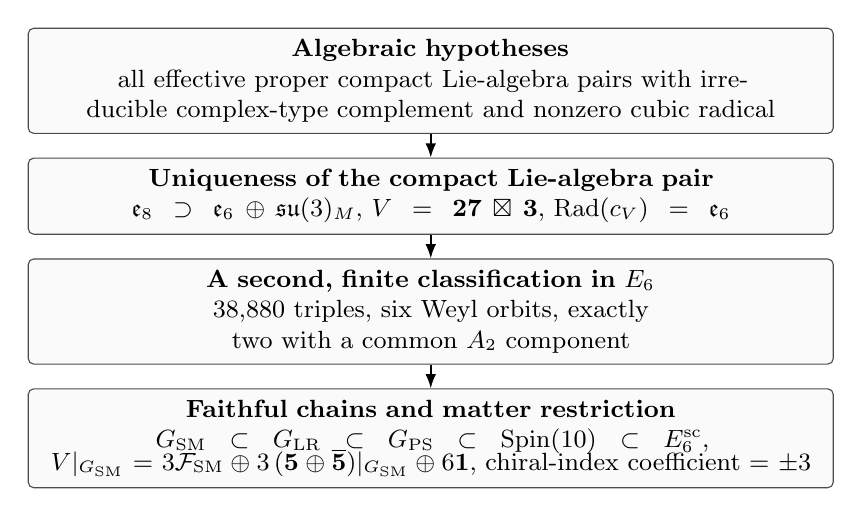
\begin{tikzpicture}[node distance=3mm]
\node[overviewbox] (domain) {\textbf{Algebraic hypotheses}\\
all effective proper compact Lie-algebra pairs with irreducible
complex-type complement and nonzero cubic radical};
\node[overviewbox,below=of domain] (pair) {\textbf{Uniqueness of the compact Lie-algebra pair}\\
\(\mathfrak e_8\supset\mathfrak e_6\oplus\mathfrak{su}(3)_M\),
\(V=\mathbf{27}\boxtimes\mathbf3\),
\(\operatorname{Rad}(c_V)=\mathfrak e_6\)};
\node[overviewbox,below=of pair] (incidence) {\textbf{A second, finite classification in \(E_6\)}\\
\(38{,}880\) triples, six Weyl orbits, exactly two with a common
\(A_2\) component};
\node[overviewbox,below=of incidence] (sm) {\textbf{Faithful chains and matter restriction}\\
\(G_{\mathrm{SM}}\subset G_{\mathrm{LR}}\subset G_{\mathrm{PS}}
\subset\operatorname{Spin}(10)\subset E_6^{\mathrm{sc}}\),\\[-1mm]
\(V|_{G_{\mathrm{SM}}}=3\mathcal F_{\mathrm{SM}}
\oplus3\,(\mathbf5\oplus\overline{\mathbf5})|_{G_{\mathrm{SM}}}
\oplus6\mathbf1\),
chiral-index coefficient \(=\pm3\)};
\draw[branch] (domain) -- (pair);
\draw[branch] (pair) -- (incidence);
\draw[branch] (incidence) -- (sm);
\end{tikzpicture}
\caption{The two classification problems. The subgroup construction uses
the two extremal orbits and the unique largest pairwise derived group. The last
coefficient records the net chiral class of the restricted module.}
\label{fig:logical-architecture}
\end{figure}

\section{Adjoint complements and cubic anomalies}

We first define complex-type complements and the cubic radical. These two
conditions specify the Lie-algebra classification problem.

Let \(\g\) be a finite-dimensional compact real Lie algebra and let
\(\h\subsetneq\g\) be a Lie subalgebra. Here compactness means that
\(\g\) admits a positive-definite ad-invariant inner product;
semisimplicity is not assumed. Write
\(\q=\g/\h\) for the quotient module and assume
\emph{effectivity}: \(\h\) contains no nonzero ideal of \(\g\). A
positive-definite \(\operatorname{ad}(\g)\)-invariant inner product gives
\[
 \q=\g/\h\simeq\h^\perp,
 \qquad \g=\h\oplus\q,
 \qquad [\h,\q]\subseteq\q.
\]
We identify the quotient with this orthogonal complement. The skew-adjoint
action of \(\h\) makes the module completely reducible. The pair
itself fixes the underlying module as \(\g/\h\).

Fraktur letters denote Lie algebras. For a representation \(R\),
\(R^*\) denotes its dual and \(\overline R\) its complex conjugate; for
compact groups these are isomorphic. We use \(R^*\) in duality statements
and bars in conventional representation labels. The symbol \(\boxtimes\)
denotes an external tensor product, and a superscript ``sc'' denotes the
simply connected compact group.

\subsection{Complex-type complements}

The algebra \(\operatorname{End}_{\h}(\q)\) consists of the real linear
maps on \(\q\) that commute with \(\h\). We require
\[
 \boxed{\ \operatorname{End}_{\h}(\q)\cong\mathbb C\ }. \tag{1}
\]
Compactness makes \(\q\) completely reducible. If it had a proper
invariant summand, projection onto that summand would be a nontrivial
idempotent in \(\operatorname{End}_{\h}(\q)\). Since \(\mathbb C\) has
no such idempotent, \(\q\) is irreducible. Choose \(J\) corresponding to
\(i\in\mathbb C\). Then \(J^2=-I\), and \(J\) is unique up to sign. Its
\(+i\)- and \(-i\)-eigenspaces in \(\q_{\mathbb C}\) are irreducible
dual \(\h\)-modules \(V\) and \(V^*\), so
\[
 \q_{\mathbb C}=V\oplus V^*,\qquad V\not\cong V^*.
\]
The two choices \(J\) and \(-J\) exchange \(V\) and \(V^*\); we call them
the two complex orientations. The Lie-algebra pair determines the unordered
dual pair \(\{V,V^*\}\), not a preferred member.

\subsection{The cubic anomaly and its radical}

The inner product on \(\q\) induces an \(\h\)-invariant Hermitian inner
product on \(V\). The operators \(\rho_V(X)\) are then skew-Hermitian,
so \(T_X=-i\rho_V(X)\) is Hermitian. With
\(\{A,B\}=AB+BA\), define
\[
\begin{aligned}
 c_V(X,Y,Z)&=\frac12\Tr_V\!\bigl(T_X\{T_Y,T_Z\}\bigr),\\
 \Phi_V(X)&=c_V(X,\cdot,\cdot),
 &\Rad(c_V)&=\ker\Phi_V.
\end{aligned}                                                       \tag{2}
\]
For a left-handed Weyl multiplet in four spacetime dimensions, \(c_V\)
is the group factor in the local triangle anomaly. Equivalently, it
polarizes the cubic trace underlying the pure-gauge term
\(\Tr_V(F^3)\) in the six-form anomaly polynomial
\cite{AlvarezGaumeGinsparg}.
The map \(\Phi_V:\h\to\operatorname{Sym}^2\h^*\) is equivariant, so
its kernel is invariant under the adjoint action and is therefore an
ideal. It is the largest ideal \(\mathfrak a\triangleleft\h\) for which
every cubic with one argument in \(\mathfrak a\) vanishes. Equivalently,
\[
 \exists\,0\ne\mathfrak k\triangleleft\h:\;
 c_V(\mathfrak k,\h,\h)=0
 \quad\Longleftrightarrow\quad \Rad(c_V)\ne0.
\]
We require
\[
                         \Rad(c_V)\ne0. \tag{3}
\]
This is the second invariant condition. For a
particular nonzero ideal \(\mathfrak k\), it is in general stronger than vanishing
only on \(\mathfrak k^3\):
\[
\begin{array}{rcl}
\text{vanishing only on \(\mathfrak k^3\)}&:&
c_V(\mathfrak k,\mathfrak k,\mathfrak k)=0,\\[1mm]
\text{vanishing with one \(\mathfrak k\)-argument}&:&
c_V(\mathfrak k,\h,\h)=0.
\end{array}                                                        \tag{4}
\]
When \(\h\) is semisimple, mixed cubics between distinct simple ideals
vanish, and the two conditions agree for a fixed ideal \(\mathfrak k\).
They need not agree when \(\h\) has a centre. The radical formulation
treats both cases uniformly and does not presuppose a choice of ideal.
Every ideal satisfying \(c_V(\mathfrak k,\h,\h)=0\) lies in
\(\Rad(c_V)\). Hence every component with one
argument in the radical vanishes, including components with arbitrary
\(\h\)-valued background insertions. Local counterterms can redistribute the
consistent anomaly among currents, but they do not alter the invariant
polynomial represented by \(c_V\) \cite{AlvarezGaumeGinsparg}. Condition (3)
applies to that invariant polynomial, not merely to a chosen subalgebra.
Duality sends \(c_V\) to \(-c_V\) and leaves its radical unchanged.

\begin{theorem}[Uniqueness of the compact Lie-algebra pair\protect\footnotemark]
\label{thm:main}
\footnotetext{For my son Noah, on his eighteenth birthday.}
Among the effective proper compact Lie-algebra pairs specified
above, conditions \textup{(1)} and \textup{(3)} have, up to isomorphism of
Lie-algebra pairs and exchange of \(V\) with \(V^*\), the unique solution
\[
 (\g,\h,\Rad(c_V),\{V,V^*\})
 =
 \bigl(\e_8,\e_6\oplus\su(3)_M,\e_6,
 \{\mathbf{27}\boxt\mathbf3,
   \overline{\mathbf{27}}\boxt\overline{\mathbf3}\}\bigr). \tag{5}
\]
Conversely, this pair satisfies the hypotheses.
\end{theorem}

\begin{remark}[Contrapositive and no-go consequence]
Every other effective proper compact Lie-algebra pair with
irreducible complex-type complement has \(\Rad(c_V)=0\). No candidate in the
full census has \(\Rad(c_V)=\mathfrak h\); the survivor is the unique case
with a proper nonzero radical. Equivalently, any different pair
must fail at least one standing hypothesis or one of conditions
\textup{(1)} and \textup{(3)}.  Group-level global forms are determined
separately in Section~4.
\end{remark}

\begin{remark}[Cubic radical and multiplicity factor]
The pair fixes \(\mathfrak h\) and \(\mathfrak q\) simultaneously.  In the
surviving case the cubic radical then separates
\(\mathfrak h=\mathfrak e_6\oplus\mathfrak{su}(3)_M\) into the
cubic-anomaly-safe ideal \(\mathfrak e_6\) and the commuting multiplicity factor
\(\mathfrak{su}(3)_M\).
\end{remark}

\begin{remark}[Invariant degrees and the surviving radical]
The basic invariant degrees of \(W(E_6)\) are
\(2,5,6,8,9,12\). The cubic trace polynomial of any
\(E_6\)-representation therefore vanishes on a Cartan subalgebra, and cubic
gauge anomalies remain zero after restriction to subgroups of \(E_6\). By
contrast, \(W(A_2)\) has invariant degrees \(2,3\). For
\(V=\mathbf{27}\boxtimes\mathbf3\), the nonzero cubic lies in the
\(SU(3)_M\) direction, while every component with an \(E_6\) insertion
vanishes. This difference in invariant degrees accounts for
\(\Rad(c_V)=\e_6\).
\end{remark}

\begin{lemma}[Structural reduction of the algebraic domain]
\label{lem:reduction}
Under the standing pair hypotheses and Conditions~\textup{(1)} and
\textup{(3)}, \(\q\) is an irreducible real
\(\h\)-module, the quotient action is faithful, \(\g\) is simple, and
\(\h\) is semisimple and maximal among proper Lie subalgebras of
\(\g\).
\end{lemma}
\begin{proof}
\emph{Maximality.}
Irreducibility was proved after (1). An intermediate algebra
\(\h\subsetneq\mathfrak l\subsetneq\g\) would then make
\(\mathfrak l/\h\) a proper nonzero \(\h\)-submodule of \(\q\).
Hence \(\h\) is maximal among proper subalgebras of \(\g\).

\emph{Faithfulness.}
Let \(\mathfrak k_0\) be the kernel of the quotient representation.
Since \(\mathfrak k_0\) acts trivially on \(\g/\h\),
\([\mathfrak k_0,\q]\subseteq\h\). But
\([\h,\q]\subseteq\q\), so this bracket lies in both summands and
vanishes. Since \(\mathfrak k_0\triangleleft\h\), this makes
\(\mathfrak k_0\) an ideal of \(\g=\h\oplus\q\) contained in \(\h\).
Effectivity therefore gives \(\mathfrak k_0=0\).
Because an element acting trivially on \(V\) also acts trivially on
\(V^*\), the \(\h\)-module \(V\) is faithful.

\emph{Simplicity of \(\g\).}
The projection of \(\mathfrak z(\g)\) to \(\q\) is fixed by \(\h\).
If it were nonzero, irreducibility would make all of \(\q\) fixed.
Every subspace would then be invariant, forcing \(\dim\q=1\); its
endomorphism algebra would be \(\mathbb R\), contrary to (1). It follows that
\(\mathfrak z(\g)\subseteq\h\).
It is an ideal of \(\g\), so effectivity gives
\(\mathfrak z(\g)=0\); compactness makes \(\g\) semisimple.

Suppose \(\g=\mathfrak g_1\oplus\mathfrak g_2\), where
\(\mathfrak g_1\) is simple and \(\mathfrak g_2\ne0\) is the sum of
the remaining simple ideals. Effectivity implies that
neither ideal is contained in \(\h\). Since \(\h\) is maximal and
each \(\mathfrak g_i\) is an ideal,
\[
 \h+\mathfrak g_1=\h+\mathfrak g_2=\g.
\]
If \(X\in\h\cap\mathfrak g_1\), write any \(Y\in\g\) as
\(Y=Y_{\h}+Y_2\), with \(Y_{\h}\in\h\) and
\(Y_2\in\mathfrak g_2\). Then \([X,Y]=[X,Y_{\h}]\in\h\), so
\(X\) acts trivially on \(\g/\h\). Faithfulness gives
\(\h\cap\mathfrak g_1=0\), and similarly
\(\h\cap\mathfrak g_2=0\). If
\(p_i:\g\to\mathfrak g_i\) are the projections, the sum identities
give surjectivity and the intersection identities give injectivity.
The restrictions \(p_i|_{\h}:\h\to\mathfrak g_i\) are therefore
isomorphisms. Since
\(\mathfrak g_1\) is simple, \(\h\) is simple, and so is
\(\mathfrak g_2\). After an automorphism the pair is
\((\mathfrak l\oplus\mathfrak l,\operatorname{diag}\mathfrak l)\).
Its quotient is the adjoint \(\mathfrak l\)-module, whose real
endomorphism algebra is \(\mathbb R\), again contradicting (1).
This contradiction proves that \(\g\) is simple.

\emph{Semisimplicity of \(\h\).}
For \(0\ne z\in\mathfrak z(\h)\), Schur's lemma gives
\(T_z=\lambda I\) for some \(\lambda\in\mathbb R\), and faithfulness
gives \(\lambda\ne0\). For \(0\ne X\in\Rad(c_V)\), faithfulness gives
\(T_X\ne0\), while equation (2) would give
\[
0=c_V(X,z,X)=\lambda\Tr_V(T_X^2),
\]
which is impossible because the nonzero Hermitian operator \(T_X\)
satisfies \(\Tr_V(T_X^2)>0\). Consequently \(\mathfrak z(\h)=0\); compactness then makes \(\h\)
semisimple.
\end{proof}

\begin{remark}[Homogeneous realization]
No closed-subgroup assumption is needed in the algebraic formulation.
By Lemma~\ref{lem:reduction}, both \(\g\) and \(\h\) are compact
semisimple Lie algebras. Let \(G^{\mathrm{sc}}\) and
\(H^{\mathrm{sc}}\) be their simply connected compact groups.
The inclusion \(\h\hookrightarrow\g\) integrates to a homomorphism
\(H^{\mathrm{sc}}\to G^{\mathrm{sc}}\). Its image \(H\) is connected
and compact, hence closed, and has Lie algebra \(\h\). Thus
\(G^{\mathrm{sc}}/H\) is an infinitesimally effective compact homogeneous
space whose isotropy module is \(\g/\h\). Conversely, every connected,
infinitesimally effective compact homogeneous pair gives the corresponding
effective Lie-algebra pair. Under (1) and (3), the two formulations
therefore classify exactly the same Lie-algebra pairs; global central
quotients are separate data.
\end{remark}

\begin{remark}[Strength of the mixed condition]
The mixed arguments are essential. If only
\(c_V(\mathfrak k,\mathfrak k,\mathfrak k)=0\) were imposed, the pairs
\(\e_6\supset\soalg(10)\oplus\mathfrak u(1)\) and
\(\e_7\supset\e_6\oplus\mathfrak u(1)\) would satisfy it for
\(\mathfrak k=\soalg(10)\) and \(\mathfrak k=\e_6\), respectively;
neither satisfies (3).
\end{remark}

\section{Exhaustive census of compact Lie-algebra pairs}

By Lemma~\ref{lem:reduction}, \(\g\) is compact and simple, \(\h\) is
maximal semisimple, and the complement is irreducible of complex type.
We separate the remaining pairs by rank. Full-rank pairs reduce to a finite
root-grading calculation. For smaller-rank \(\h\), index arithmetic excludes
the exceptional ambient algebras, and a uniform highest-weight argument
excludes the classical ones.

We use \(A_n=\su(n+1)\).  A subalgebra is called regular when it is normalised
by a Cartan subalgebra of \(\g\).

\subsection{The full-rank branch}

A regular maximal subalgebra has full rank.  Indeed, if
\(\operatorname{rank}\h<\operatorname{rank}\g\), regularity supplies a
nonzero toral subalgebra \(\mathfrak t_0\subset C_\g(\h)\), and
\[
 \h\subsetneq \h+\mathfrak t_0\subsetneq\g,
\]
contrary to maximality.  Conversely, any equal-rank subalgebra contains a
maximal torus of \(\g\) and is regular.

\begin{lemma}[Saturation of a closed root subsystem]
\label{lem:closed-subsystem-saturation}
If \(\Psi\subseteq\Phi\) is a closed root subsystem, then
\[
 \Phi\cap\mathbb Z\Psi=\Psi.
\]
In particular, if \(\Psi\subsetneq\Phi\), then
\(\mathbb Z\Psi\ne\mathbb Z\Phi\).
\end{lemma}
\begin{proof}
Let \(\alpha\in\Phi\cap\mathbb Z\Psi\).  Write
\(\alpha=\beta_1+\cdots+\beta_m\), with each \(\beta_j\in\Psi\), and choose
such an expression with \(m\) minimal; negative coefficients may be absorbed
by replacing roots of \(\Psi\) with their negatives.  The claim is immediate
for \(m=1\).  If \(m>1\), then
\[
 (\alpha,\alpha)=\sum_{j=1}^m(\alpha,\beta_j)>0,
\]
so \((\alpha,\beta_j)>0\) for some \(j\).  If \(\alpha=\beta_j\), then
\(\alpha\in\Psi\).  Otherwise the root-string property gives
\(\alpha-\beta_j\in\Phi\).  This root lies in \(\mathbb Z\Psi\) and is a sum
of \(m-1\) roots of \(\Psi\), hence belongs to \(\Psi\) by induction.
Closedness of \(\Psi\) then gives
\(\alpha=(\alpha-\beta_j)+\beta_j\in\Psi\).  Thus
\(\Phi\cap\mathbb Z\Psi\subseteq\Psi\); the reverse inclusion is immediate.
If \(\mathbb Z\Psi=\mathbb Z\Phi\), the displayed equality gives
\(\Phi=\Psi\), proving the final assertion.
\end{proof}

\begin{lemma}[Complex type and cyclic root gradings]
\label{lem:cyclic-root-grading}
Suppose \(\operatorname{rank}\h=\operatorname{rank}\g\).  Then the root
spaces of \(\g_{\mathbb C}\) relative to a common Cartan subalgebra admit
one of the following two gradings:
\[
 \g_{\mathbb C}=\h_{\mathbb C}\oplus\g_1
 \quad (\mathbb Z_2),
 \qquad\text{or}\qquad
 \g_{\mathbb C}=\h_{\mathbb C}\oplus\g_1\oplus\g_2
 \quad (\mathbb Z_3),
\]
where in the second case \(\g_1\cong V\), \(\g_2\cong V^*\), and
\([\g_i,\g_j]\subseteq\g_{i+j}\).  The involutive case has a
self-conjugate quotient and therefore cannot satisfy condition~\textup{(1)}.
\end{lemma}
\begin{proof}
Let \(\Phi\) be the root system of \(\g_{\mathbb C}\), let \(\Psi\) be the
root subsystem of \(\h_{\mathbb C}\), and put
\(Q=\mathbb Z\Phi\), \(L=\mathbb Z\Psi\).  Root operators of \(\h\) change
weights by elements of \(L\).  Since \(V\) is irreducible, all roots whose
root spaces lie in \(V\) have one class \(c\in Q/L\); those in \(V^*\)
have class \(-c\).  Every root therefore has class \(0,c\), or \(-c\), and
these classes generate \(Q/L\).  Since \(\Psi\) is proper and closed,
Lemma~\ref{lem:closed-subsystem-saturation} gives \(Q/L\ne0\).  Hence
\(c\ne0\).

If \(2c=0\), the quotient is the odd part of an inner involution.  Compact
conjugation preserves that odd root set because \(-c=c\).  For a classical
ambient algebra, an inner involution either has a unitary block centralizer
with nonzero center, or has an orthogonal or symplectic block centralizer whose
odd module is a self-dual tensor product.  For an exceptional ambient algebra,
the finite involutive calculation described in
Proposition~\ref{prop:direct-toral-census} shows that
whenever the fixed algebra is semisimple, the odd weight graph is connected.
In every case compatible with semisimplicity the irreducible odd module is
self-conjugate, not of complex type.

Assume now that \(2c\ne0\).  If \([V,V]=0\), compact conjugation also gives
\([V^*,V^*]=0\), while the root classes give
\([V,V^*]\subseteq\h_{\mathbb C}\).  The map acting as \(0,+1,-1\) on
\(\h_{\mathbb C},V,V^*\), respectively, is then a nonzero derivation of the
simple algebra \(\g_{\mathbb C}\).  It is inner and centralizes
\(\h_{\mathbb C}\).  But \(\h\) is semisimple of full rank, so its roots
span the dual of the common Cartan and its centralizer in \(\g_{\mathbb C}\)
is zero, a contradiction.  Hence \([V,V]\ne0\).  A nonzero bracket has root
class \(2c\), which must be one of \(0,c,-c\).  The first possibility is
excluded by \(2c\ne0\), and the second would give \(c=0\).  Thus
\(2c=-c\), so \(3c=0\).  The quotient map \(Q\to Q/L\cong\mathbb Z_3\)
defines a toral order-three automorphism with fixed algebra
\(\h_{\mathbb C}\) and the asserted grading.
\end{proof}

\begin{proposition}[Direct toral grading census]
\label{prop:direct-toral-census}
Let \((\g,\h)\) satisfy the standing pair hypotheses and
Conditions~\textup{(1)} and~\textup{(3)}, with
\(\operatorname{rank}\h=\operatorname{rank}\g\).
The pair must be isomorphic to exactly one of the six candidates below.
Here condition~\textup{(3)} has been used through
Lemma~\ref{lem:reduction} to establish semisimplicity of \(\h\);
the cubic coefficients are evaluated in Table~\ref{tab:direct-census}.
\[
 \mathfrak g_2\supset A_2,\quad
 \mathfrak f_4\supset A_2+A_2,\quad
 \e_6\supset A_2^3,\quad
 \e_7\supset A_5+A_2,\quad
 \e_8\supset A_8,\quad
 \e_8\supset E_6+A_2.
\]
Their complex halves have dimensions
\[
 3,\quad18,\quad27,\quad45,\quad84,\quad81,
\]
respectively, and are irreducible and inequivalent to their duals.
\end{proposition}
\begin{proof}
For the classical groups the calculation is immediate in the defining
module.  A nonidentity inner automorphism of order three of \(\mathfrak{su}(n)\)
has a representative with eigenvalues among \(c,c\zeta,c\zeta^2\), where
\(\zeta^3=1\), \(\zeta\ne1\); the representative need not have order three.
If \(s\ge2\) eigenspaces are nonempty, its centralizer
\(S(\prod_{j=1}^{s}U(n_j))\) has center dimension \(s-1>0\).
In \(SO(n)\) and \(Sp(n)\), an order-three inner automorphism admits an
order-three representative, since their centers have order coprime to three.
A nonidentity such representative has a
unitary factor in its centralizer, again giving a center.  Thus no proper
classical fixed algebra is semisimple.  For involutions, the semisimple
classical centralizers have self-dual tensor-product quotients.

For the exceptional groups the remaining calculation is finite. Starting
from each Cartan matrix, simple reflections generate the roots in
simple-root coordinates. A homomorphism \(Q\to\mathbb Z_m\), \(m=2,3\),
is determined by its values on the simple roots. We enumerate all
\(m^{\operatorname{rank}\g}-1\) nonzero assignments and form their Weyl
orbits. This covers every toral grading under consideration. We retain the
gradings whose grade-zero roots span the full rank and test connectedness
of the grade-one weight graph. The exact implementation and resulting
root data are supplied in the computational companion \cite{ComputationalCompanion}.
Its vertices are the roots of degree one; two are joined when their
difference is a grade-zero root. The corresponding root operator acts
nontrivially between their one-dimensional weight spaces. Since the
grade-zero algebra contains the full Cartan subalgebra, its submodules are
sums of these weight spaces, and the connected components are precisely the
irreducible constituents. For
\(m=2\) every semisimple row has a connected self-conjugate odd module.  For
\(m=3\) the six rows displayed above are the complete list.  The Killing
form pairs grades one and two nondegenerately, so the two modules are dual;
the connected grade-one graphs prove irreducibility.
\end{proof}

\begin{lemma}[Degree-three invariant theory]
\label{lem:degree-three-invariant}
For a simple complex Lie algebra \(\mathfrak s\),
\[
 \bigl(\operatorname{Sym}^3\mathfrak s^*\bigr)^{\mathfrak s}\ne0
 \quad\Longleftrightarrow\quad
 \mathfrak s\text{ has type }A_n\text{ with }n\ge2.
\]
Thus only type \(A\) factors can carry a nonzero perturbative cubic
coefficient; a particular representation of such a factor may still have
coefficient zero.
\end{lemma}
\begin{proof}
By Chevalley's theorem, invariant polynomials on \(\mathfrak s\) have basic
degrees equal to the exponents plus one.  Degree three occurs precisely in
type \(A_n\), \(n\ge2\).
\end{proof}

\subsection{The rank-deficient branch}

No classification of maximal subalgebras is needed in this branch.  The
exceptional ambient algebras are excluded by a finite arithmetic sieve; the
classical ambient algebras admit a uniform highest-weight argument.

\begin{proposition}[Exceptional rank-deficient no-go]
\label{prop:exceptional-rankdef}
Let \(\g\) be exceptional simple and let \(\h\subset\g\) be semisimple with
\(\operatorname{rank}\h<\operatorname{rank}\g\).  If
\((\g/\h)_{\mathbb C}=V\oplus V^*\) with \(V\) irreducible of complex type,
then \(\Rad(c_V)=0\).
\end{proposition}
\begin{proof}
Write \(\h=\bigoplus_i\h_i\) and
\(V=\boxtimes_i V_i\).  Let \(d_i=\dim V_i\).  Normalize the quadratic
index by taking long roots to have squared length two and requiring
\(T(\operatorname{ad}_{\h_i})=h_i^\vee\); in particular
\(T_{A_{n-1}}(\mathbf n)=\tfrac12\).  If \(I_i\in\mathbb Z_{>0}\) is the
Dynkin index of \(\h_i\hookrightarrow\g\), restriction of the adjoint
representation gives the necessary equations
\[
 \dim\g=\sum_i\dim\h_i+2\prod_i d_i,
 \qquad
 h_\g^\vee I_i=h_i^\vee+2T_i\prod_{j\ne i}d_j. \tag{6}
\]
The normalisation is visible in the surviving full-rank row.  For
\(E_8\supset E_6+A_2\), both embeddings have index one and
\[
 30=12+2\cdot3\cdot3,
 \qquad
 30=3+2\cdot\frac12\cdot27. \tag{6a}
\]
The radical is nonzero only if at least one simple factor has vanishing cubic
coefficient on \(V_i\); Lemma~\ref{lem:degree-three-invariant} makes this
condition automatic for every non-\(A\) factor.

The dimension equation bounds the representation search before any index is
computed.  Since \(\h\ne0\) is semisimple, rank deficient, and
\(\dim\g-\dim\h=2\dim V\), the smallest parity-compatible possibility for
\(\dim\h\) gives
\[
\begin{array}{c|ccccc}
 \g&G_2&F_4&E_6&E_7&E_8\\
\hline
 \text{smallest compatible }\dim\h&\text{none}&6&6&3&6\\
 \max\dim V&\text{none}&23&36&65&121.
\end{array} \tag{6b}
\]
For \(G_2\), the only smaller-rank semisimple type is \(A_1\), and
\(14-3\) is odd.  For the even-dimensional ambient algebras the smallest
parity-compatible semisimple dimension is six, while \(E_7\) admits
\(A_1\) of dimension three.

There are finitely many multisets of simple factor types of smaller total
rank. For each factor, enumerate dominant Dynkin labels from zero by
successively increasing one label. Weyl's dimension formula is strictly
increasing in each label, so a branch may be stopped when its dimension
exceeds the applicable bound in \textup{(6b)}. This terminates and includes
every admissible highest weight. Each factor dimension is at most
\(\dim V\), so the same bounds suffice for every factor.

For every multiset, form all representation products within these bounds,
identify permutations of identical factors, and impose the dimension
equation, complex type, a zero cubic coefficient on at least one factor,
and positive integrality of every index in \textup{(6)}. The finite
calculation leaves no candidate in any of the five ambient types
\cite{ComputationalCompanion}. Its machine-readable audit records every
product reaching the index test and the nonintegral index excluding it.
These are necessary conditions on an embedding; their empty intersection
is sufficient for the no-go conclusion.
\end{proof}

\begin{lemma}[Defining modules and canonical constituents]
\label{lem:classical-constituents}
Let \(\g_{\mathbb C}\) be \(\mathfrak{sl}(W)\),
\(\mathfrak{so}(W)\), or \(\mathfrak{sp}(W)\), and suppose
\(\h_{\mathbb C}\subset\g_{\mathbb C}\) is semisimple and maximal with
quotient \(V\oplus V^*\), where \(V\not\cong V^*\) is irreducible.  Then
\(W\) is irreducible as an \(\h_{\mathbb C}\)-module and
\(\h_{\mathbb C}\) is simple.

If \(\lambda\) is the highest weight of \(W\), let \(\lambda^*\) be the
highest weight of \(W^*\), and write \(i\mapsto i^*\) for the Dynkin-node
involution induced by duality.  The following constituents occur with
multiplicity one:
\[
 V_{\lambda+\lambda^*}\subset W\otimes W^*,\qquad
 V_{2\lambda}\subset\operatorname{Sym}^2W,
\]
and, when \(W\) is orthogonal,
\[
 V_{2\lambda-\alpha_i}\subset\Lambda^2W
 \quad\text{for every }i\text{ with }
 \langle\lambda,\alpha_i^\vee\rangle>0. \tag{6c}
\]
If the last integer is at least three, then
\(V_{2\lambda-3\alpha_i}\) also occurs in \(\Lambda^2W\).
\end{lemma}
\begin{proof}
\emph{Irreducibility of \(W\).}
Suppose first that the defining module is reducible.  In the compact
real form, complete reducibility gives either a proper invariant orthogonal
decomposition or
an irreducible real module whose complexification splits as an isotropic
dual pair.  In the first case let \(B\) be the compact block stabilizer.  If
\(\h\subsetneq B\), maximality is contradicted.  If \(\h=B\), then in the
unitary case \(B\) has nonzero center, contrary to semisimplicity; in the
orthogonal and symplectic cases the off-diagonal quotient is a sum of
self-dual tensor products of defining blocks, contrary to irreducible complex
type.  Under the isotropic-dual-pair alternative, the splitting defines an \(\h\)-invariant
orthogonal complex structure, and \(\h\) lies in its proper compact unitary
centralizer, whose nonzero centre excludes equality with the semisimple
\(\h\), again contradicting maximality. Thus the defining module is
irreducible.

\emph{Simplicity of \(\h\).}
Write \(W=\boxtimes_iW_i\) for the simple ideals of \(\h\). In
\(\mathfrak{sl}(W)\), two distinct factors produce the self-dual constituent
\(\operatorname{ad}\h_i\boxtimes\operatorname{ad}\h_j\) outside \(\h\).
In the orthogonal or symplectic cases every \(W_i\) is self-dual.
Choose its invariant nondegenerate bilinear form, symmetric or alternating
as appropriate. Adjointness in the decomposition
\(\operatorname{End}(W_i)=K_i\oplus P_i\) refers to this bilinear form:
\(K_i\) is the skew-adjoint part and \(P_i\) the self-adjoint part. With \(P_i^0=\{p\in P_i:\operatorname{Tr}p=0\}\) for the traceless
self-adjoint part, the ambient Lie algebra is the odd-parity part of
\(\bigotimes_i(K_i\oplus P_i)\).  Three factors again give the self-dual
constituent
\(\operatorname{ad}\h_1\boxtimes\operatorname{ad}\h_2
 \boxtimes\operatorname{ad}\h_3\).  With two factors, the nonzero blocks
\(\operatorname{ad}\h_1\boxtimes P_2^0\) and
\(P_1^0\boxtimes\operatorname{ad}\h_2\) lie in disjoint tensor summands
outside \(\h\) and are self-dual by their nondegenerate trace pairings.
But \(V\oplus V^*\) has no nonzero proper self-dual submodule, so it cannot
contain both blocks.  If \(P_1^0=0\), then \(W_1\) is two-dimensional
symplectic.  When \(P_2^0\ne0\), maximality forces \(\h_2=K_2\), and the
quotient is \(\operatorname{ad}\mathfrak{sl}_2\boxtimes P_2^0\), an
irreducible self-dual module; if both traceless parts vanish, the quotient is
zero.  Hence \(\h\) is simple.

\emph{Highest-weight constituents.}
The first two displayed inclusions are the Cartan products. For the third,
if \(v_\lambda\) is a highest-weight vector and \(f_i\) a simple lowering
operator, then
\(v_\lambda\wedge f_iv_\lambda\) is a highest-weight vector of weight
\(2\lambda-\alpha_i\). The corresponding weight space in \(\Lambda^2W\)
is one-dimensional, which proves the stated multiplicity. If
\(m=\langle\lambda,\alpha_i^\vee\rangle\ge3\), the vector
\[
 m\,v_\lambda\wedge f_i^3v_\lambda
 -3(m-2)f_iv_\lambda\wedge f_i^2v_\lambda
\]
is nonzero and highest of weight \(2\lambda-3\alpha_i\).  In the remaining
dual-node cases, this weight and its dual are distinct from the adjoint and
from the pair \(2\lambda-\alpha_i,2\lambda-\alpha_{i^*}\); they therefore
supply an additional quotient pair.
\end{proof}

\begin{proposition}[Classical rank-deficient no-go]
\label{prop:classical-rankdef}
Let \((\g,\h)\) satisfy the standing pair hypotheses, let \(\g\) be classical
simple, and let \(\h\subset\g\) be rank deficient. Under
condition~\textup{(1)}, the radical of the complex half is zero.
\end{proposition}
\begin{proof}
Assume for contradiction that \(\Rad(c_V)\ne0\).  Then the standing pair
hypotheses, condition~\textup{(1)}, and Lemma~\ref{lem:reduction} imply
that \(\h\) is semisimple and maximal, so
Lemma~\ref{lem:classical-constituents} applies; use its notation.  If
\(\g_{\mathbb C}=\mathfrak{sl}(W)\), the self-dual Cartan constituent
\(V_{\lambda+\lambda^*}\) must be the adjoint module of \(\h\); otherwise it
would be a self-dual summand of the quotient.  Thus
\(\lambda+\lambda^*=\theta\), where \(\theta\) is the highest root of
\(\h_{\mathbb C}\).  The three Cartan-product equations used in
this proof are labelwise, and their nonzero dominant solutions are
\[
\begin{array}{@{}ll@{}}
\lambda+\lambda^*=\theta
 & A_r:\ \omega_1,\omega_r;\quad C_r:\ \omega_1
   \ \text{(equivalently }B_2:\ \omega_2\text{)},\\[1mm]
2\lambda=\theta
 & C_r:\ \omega_1
   \ \text{(including }A_1,\text{ and equivalently }B_2:\ \omega_2\text{)},\\[1mm]
2\lambda-\alpha_i=\theta,\ i=i^*
 & A_1:\ 2\omega_1;\ A_3:\ \omega_2;\ B_r:\ \omega_1;   B_3:\ \omega_3;\ C_2:\ \omega_2;\\[-1mm]
 & D_r:\ \omega_1;\ D_4:\ \omega_3,\omega_4;\ G_2:\ \omega_1.
\end{array} \tag{6d}
\]
In the symplectic case, \(\g_{\mathbb C}\cong\operatorname{Sym}^2W\),
and the self-dual Cartan constituent \(V_{2\lambda}\) must likewise be the
adjoint of \(\h\). This gives the second equation, \(2\lambda=\theta\).
The first row gives the standard \(A_r\) representation, for which the
ambient algebra equals \(\h\), and the defining symplectic representation,
whose quotient in \(\mathfrak{sl}(W)\) is self-dual.  The second row gives
only the standard symplectic algebra and low-dimensional isomorphisms, so
\(\mathfrak{sp}(W)\) has no proper complex-type quotient.

Suppose \(\g_{\mathbb C}=\mathfrak{so}(W)\).  For every support node fixed by
duality, the constituent in \textup{(6c)} is self-dual and must equal the
adjoint, so \(2\lambda-\alpha_i=\theta\).  The third row of
\textup{(6d)} consists of defining representations and low-rank
isomorphisms, together with \(G_2\subset SO(7)\) and the spin embedding
\(B_3\subset SO(8)\); their quotients are zero or self-dual.
For distinct support nodes, the weights \(2\lambda-\alpha_i\) are
distinct. Once the self-dual cases have been excluded, each must be one of
the two quotient highest weights. There can therefore be only one pair of
support nodes exchanged by duality. Their coefficients are equal because
the orthogonal module \(W\) is self-dual. Write this common coefficient as
\(a\). Such a pair occurs only in types \(A_r\), odd \(D_r\), and \(E_6\).

For \(A_{N-1}\), choose the pair \(i,N-i\) with \(1\le i<N/2\).
For a highest weight \(\mu=\sum_{j=1}^{N-1}b_j\omega_j\), put
\(\ell_j=\sum_{k=j}^{N-1}b_k\), \(\ell_N=0\), and
\(x_j=\ell_j+N-j\). We use the cubic Harish--Chandra normalisation
\[
 C_3(\mu)=\sum_{j=1}^N(x_j-\bar x)^3,\qquad
 \bar x=\frac1N\sum_{j=1}^N x_j.
\]
In this normalisation the constituent \(\mu_i=2\lambda-\alpha_i\) has
\[
 C_3(\mu_i)=-6a\bigl(2a+N-2i\bigr)\ne0. \tag{6e}
\]
For completeness, let \(u,v\) be the \(i\)-th and \((i+1)\)-st centred
coordinates of \(2\lambda\). Self-duality makes their full cubic sum zero,
while
\[
 u-v=2a+1,\qquad u+v=2a+N-2i.
\]
Subtracting \(\alpha_i\) changes only these two centred coordinates, to
\(u-1,v+1\). Hence the change in the cubic sum is
\[
 (u-1)^3-u^3+(v+1)^3-v^3
 =3(u+v)(v-u+1)=-6a(2a+N-2i),
\]
which proves \textup{(6e)}. In type \(A\), the cubic trace tensor is a
multiple of the unique invariant cubic. Contracting it with that invariant
yields the cubic central eigenvalue times the dimension, up to a fixed
nonzero normalisation. Thus its coefficient vanishes exactly when
\(C_3\) does. The constituent \(\mu_i\) is consequently a quotient half
with nonzero cubic index, so the radical is zero.

For odd \(D_r\) and for \(E_6\), a coefficient \(a\ge3\) gives the additional
constituent \(V_{2\lambda-3\alpha_i}\), contradicting the assumption that
the quotient has only one dual pair.  It remains to inspect \(a=1,2\).  Put
\[
 D_{r,a}=\dim V_{a(\omega_{r-1}+\omega_r)},\qquad
 M_{r,a}=\dim V_{2a(\omega_{r-1}+\omega_r)-\alpha_{r-1}}.
\]
For odd \(r\ge5\) and \(a\in\{1,2\}\), we will show
\[
 \binom{D_{r,a}}2>r(2r-1)+2M_{r,a}.
\]
Thus the adjoint and the proposed dual pair cannot exhaust \(\Lambda^2W\).
Weyl's formula gives the ratios
\[
 \frac{4M_{r,1}}{D_{r,1}^2}
 =\frac{36(r-1)(2r+1)}{r(r+2)(r+3)(r+4)},
\]
\[
 \frac{4M_{r,2}}{D_{r,2}^2}
 =\frac{5{,}376{,}000(r-1)(r+2)(2r+1)(2r+3)^2(2r+5)}
 {r(r+1)(r+3)^2(r+4)^3(r+5)^3(r+6)^2(r+7)(r+8)}.
\]
Set \(R_{r,a}=4M_{r,a}/D_{r,a}^2\).  The two sequences decrease for
\(r\ge5\).  Indeed, after clearing the positive denominators in
\(R_{r+1,a}/R_{r,a}<1\) and writing \(n=r-5\), the two differences are
\[
 4n^3+57n^2+259n+365
\]
and
\[
\begin{aligned}
 &32n^7+1{,}624n^6+34{,}692n^5+404{,}090n^4\\
 &\quad+2{,}769{,}860n^3+11{,}162{,}622n^2
      +24{,}455{,}216n+22{,}419{,}744,
\end{aligned}
\]
respectively.  Hence
\[
 R_{r,1}\le R_{5,1}=\frac{22}{35}<\frac23,
 \qquad
 R_{r,2}\le R_{5,2}=\frac{1274}{8019}<\frac16.
\]
Moreover
\(D_{r,1}=\binom{2r}{r-1}\ge r(2r-1)\), and monotonicity in the highest
weight gives \(D_{r,2}>D_{r,1}\).  Writing \(H=r(2r-1)\), we obtain
\[
\begin{aligned}
 \binom{D_{r,1}}2-H-2M_{r,1}
 &\ge \frac{H(H-9)}6>0,\\
 \binom{D_{r,2}}2-H-2M_{r,2}
 &\ge \frac{H(5H-18)}{12}>0.
\end{aligned}
\]
Thus \(\Lambda^2W\) contains more than the adjoint and one dual pair.  For
\(E_6\), the two possible supports are
\(\{\omega_1,\omega_6\}\) and \(\{\omega_3,\omega_5\}\); the four remaining
values \(a=1,2\) give the positive dimension gaps
\[
 52{,}897,\quad3{,}008{,}865{,}288,
 \quad1{,}949{,}250{,}433,
 \quad24{,}307{,}954{,}884{,}506{,}865.
\]
These four dimension gaps follow from Weyl's product formula; their exact
values and a separate check of the symbolic inequalities above are recorded
in the computational companion \cite{ComputationalCompanion}.
The inequalities are uniform in rank; the finite regression tests supplied
with the code are supplementary checks, not the all-rank argument.
No rank-deficient classical pair can have a nonzero radical.
\end{proof}

\subsection{Cubic indices and the survivor}

For a simple factor of type \(A_{N-1}\) with \(N\ge3\), let \(A(R)\) be the
cubic index, normalised by \(A(\mathbf N)=1\); for \(A_1\) and every other simple type put
\(A(R)=0\).  Duality gives \(A(R^*)=-A(R)\), and for
\(V=\boxtimes_iV_i\) the coefficient on the \(i\)-th factor is
\[
 A_i(V)=A(V_i)\prod_{j\ne i}\dim V_j. \tag{6f}
\]
Write \(\mathbf A(V):=(A_i(V))_i\).
Mixed cubics between distinct simple ideals vanish because they factor
through the trace of a generator.  Hence \(\Rad(c_V)\) is the sum of the
simple ideals whose coefficients in \textup{(6f)} vanish.

Table~\ref{tab:direct-census} gives the cubic coefficients of the six
full-rank rows in Proposition~\ref{prop:direct-toral-census}.
\begin{table}[!t]
\centering
\caption{The direct full-rank census and its cubic coefficients.  The
radical is the sum of the factors with zero coefficient.}
\label{tab:direct-census}
\small
\renewcommand{\arraystretch}{1.12}
\setlength{\tabcolsep}{5pt}
\begin{tabular}{@{}llll@{}}
\toprule
pair \(\g\supset\h\) & complex summand \(V\) & \(\mathbf A(V)\) &
\(\Rad(c_V)\)\\
\midrule
\(\mathfrak g_2\supset\su(3)\)
 & \(\mathbf3\) & \(1\) & \(0\)\\
\(\mathfrak f_4\supset\su(3)\oplus\su(3)\)
 & \(\mathbf6\boxt\overline{\mathbf3}\) & \((21,-6)\) & \(0\)\\
\(\e_6\supset\su(3)^{\oplus3}\)
 & \(\mathbf3\boxt\mathbf3\boxt\mathbf3\) & \((9,9,9)\) & \(0\)\\
\(\e_7\supset\su(6)\oplus\su(3)\)
 & \(\mathbf{15}\boxt\overline{\mathbf3}\) & \((6,-15)\) & \(0\)\\
\(\e_8\supset\su(9)\)
 & \(\Lambda^3\mathbf9\) & \(9\) & \(0\)\\
\(\e_8\supset\e_6\oplus\su(3)_M\)
 & \(\mathbf{27}\boxt\mathbf3\) & \((0,27)\) & \(\e_6\)\\
\bottomrule
\end{tabular}
\end{table}

The entries follow from the standard cubic-index formulas
\cite{Slansky,McKayPatera}: for \(N\ge3\) and \(1\le k\le N-1\),
\[
 A(\Lambda^k\mathbf N)
 =\frac{(N-2k)(N-3)!}{(k-1)!(N-k-1)!},
 \qquad
 A(\operatorname{Sym}^2\mathbf N)=N+4,
\]
and the tensor-product rule \textup{(6f)}; the trivial exterior powers at
\(k=0,N\) have index zero.  The Lie algebra \(E_6\) has no
invariant symmetric cubic, whereas \(A_2\) does.  The order-three grading
produces the pair \(E_6+A_2\); degree-three invariant theory distinguishes
the anomalous factor from the radical.  Thus the last row has
\[
 \mathbf A(V)=(0,27),\qquad \Rad(c_V)=\e_6.
\]
The cubic on the \(\mathbf{27}\) is a trilinear form on the representation;
the vanishing used here concerns invariant trilinear forms on the Lie algebra
\(\e_6\).

\begin{proof}[Proof of Theorem~\ref{thm:main}]
Lemma~\ref{lem:reduction} places every pair in the algebraic domain
into the same structural normal form.
Lemma~\ref{lem:cyclic-root-grading} and
Proposition~\ref{prop:direct-toral-census} give the complete full-rank branch;
Table~\ref{tab:direct-census} leaves only its final row.
Propositions~\ref{prop:exceptional-rankdef} and~
\ref{prop:classical-rankdef} exclude every rank-deficient pair with nonzero
radical.  The final row satisfies all hypotheses, proving the converse.
\end{proof}

\begin{remark}[Completeness of the classification]
The proof uses no classification of maximal subalgebras or homogeneous
spaces.  The full-rank branch is a finite toral-grading census from Cartan
matrices; the exceptional rank-deficient branch is a finite
Weyl-dimension/index sieve; and the classical rank-deficient branch is the
uniform highest-weight argument above. The manuscript proves the reductions
and establishes their completeness; the accompanying programs perform the
remaining finite calculations.
\end{remark}


\subsection{The centralizer and multiplicity three}
For the unique pair, the radical and its centralizer are
\[
 \Rad(c_V)=\e_6,
 \qquad C_{\h}(\Rad(c_V))=\su(3)_M.
\]
Here \(C_{\h}\) denotes the centralizer in \(\h\). The radical is the
largest ideal on which all cubic coefficients, including mixed ones, vanish.
Its centralizer acts on the second tensor factor, and its defining
\(\mathbf3\) gives three copies of the \(\mathbf{27}\) after restriction to
\(E_6\). The subscript \(M\) records this multiplicity.
Section~5 computes the cubic on this factor. The adjoint branching
displays \(V\) and \(V^*\) as the two halves of the adjoint complement:
\begin{equation}
\tag{7}
\mathbf{248}=(\mathbf{78},\mathbf1)\oplus(\mathbf1,\mathbf8)
 \oplus(\mathbf{27},\mathbf3)
 \oplus(\overline{\mathbf{27}},\overline{\mathbf3}).
\label{eq:e8branch}
\end{equation}
Restriction to the first factor gives
\(V|_{E_6^{\mathrm{sc}}}=3\,\mathbf{27}\) and
\(V^*|_{E_6^{\mathrm{sc}}}=3\,\overline{\mathbf{27}}\). Either orientation
therefore has multiplicity three.

\subsection{The global exceptional subgroup}
The same branching also determines the global image inside \(E_8\). The
Lie-algebra inclusion integrates to a homomorphism
\(\varphi:E_6^{\mathrm{sc}}\times SU(3)_M\to E_8\) with finite central
kernel. Choose generators \(z_E\in Z(E_6^{\mathrm{sc}})\) and
\(z_3\in Z(SU(3)_M)\) that act by the same primitive cube root
\(\zeta_3\) on
\(\mathbf{27}\) and \(\mathbf3\). The adjoint decomposition
\eqref{eq:e8branch} shows that
\(\langle(z_E,z_3^{-1})\rangle\) acts trivially on every summand.
Conversely, a central kernel element lies in the product of the two
order-three centers, and its action on
\(\mathbf{27}\boxt\mathbf3\) forces it into this diagonal subgroup.
Faithfulness of the adjoint representation of \(E_8\) leaves the kernel
\(\langle(z_E,z_3^{-1})\rangle\). The global subgroup is
\[
 \frac{E_6^{\mathrm{sc}}\times SU(3)_M}
 {\langle(z_E,z_3^{-1})\rangle}\subset E_8.
\]
The image of \((z_E,1)\) acts on
\(\h_{\mathbb C},V,V^*\) with eigenvalues
\(1,\zeta_3,\zeta_3^{-1}\), respectively, and realizes
\eqref{eq:e8branch} as a \(\mathbb Z/3\)-grading. The branching is
classical \cite{Slansky,BarsGunaydin}; the classification above shows
that it is the only row satisfying (1) and (3).

\section{Extremal intersections in \texorpdfstring{\(E_6\)}{E6}}
\label{sec:incidence}

The Lie-algebra classification leaves a single embedded
\(E_6^{\mathrm{sc}}\), up to \(E_8\)-conjugacy. Theorem~\ref{thm:main} fixes the pair \(E_6+A_2\subset E_8\) up to automorphisms of \(\e_8\), and all automorphisms of compact \(\e_8\) are inner.

We now work inside this \(E_6\). Closed root subsystems determine connected
regular subgroups, and their intersections determine the semisimple roots of
common connected subgroups. Choosing one maximal proper subsystem from each
Weyl orbit gives a finite configuration space. We study two Weyl-invariant
questions on it: simultaneous pairwise maximality and maximal common
intersection.

The calculation rests on three pairwise facts. A \(D_5\)--\((A_5+A_1)\)
intersection has two possible types; the \(D_5\)--\(A_2^3\) intersection
always has type \(A_2+A_1+A_1\); and an \((A_5+A_1)\)--\(A_2^3\)
intersection is large precisely when
the distinguished root pair lies in the \(A_2^3\) subsystem. The two
extremal theorems combine these facts in different ways.

\subsection{The finite configuration space}

The three maximal subsystem types admit concrete parametrisations that make
the finite problem explicit. Fix a maximal torus \(T_0\subset E_6^{\mathrm{sc}}\)
with Lie algebra \(\mathfrak t_0\), let \(\Phi=\Phi(E_6)\), and write
\(\mathcal W=W(E_6)\). We use Bourbaki numbering: the chain is
\(1-3-4-5-6\), with node \(2\) attached to node \(4\). The Cartan matrix
has diagonal entries \(2\), entries \(-1\) on these edges, and zero
elsewhere. A subsystem
\(\Psi\subseteq\Phi\) is \emph{closed} when
\[
 \alpha,\beta\in\Psi,\quad \alpha+\beta\in\Phi
 \quad\Longrightarrow\quad \alpha+\beta\in\Psi.
\]
For such \(\Psi\), let \(\widehat\Psi\) be the connected regular
subgroup containing \(T_0\) with
\[
 \operatorname{Lie}(\widehat\Psi)_{\mathbb C}
 =(\mathfrak t_0)_{\mathbb C}
  \oplus\bigoplus_{\beta\in\Psi}(\e_6)_{\beta}.
\]

The intersections of these regular groups retain the common maximal torus
\(T_0\). Passing to the derived subgroup retains only the torus generated
by the common coroots; after the third intersection, some of these
directions can become central.
For two subsystems \(P,Q\), define
\[
 H_{PQ}=[(\widehat P\cap\widehat Q)^\circ,
          (\widehat P\cap\widehat Q)^\circ].
\]
Here the superscript \(\circ\) denotes the identity component, and
\([L,L]\) is the derived subgroup of \(L\).
The group \(H_{PQ}\) is the semisimple intermediate group obtained by
intersecting two regular groups and taking the derived subgroup. We then
intersect this intermediate group with the third regular group and take the identity
component. This is the \emph{pair-first construction}. The derived-subgroup
step makes the choice of the first pair matter. We choose the pair whose
intermediate group has greatest dimension; Proposition~\ref{prop:largest-intermediate}
proves that this choice is unique for every triple.

\begin{proposition}[Maximal closed subsystems of \(E_6\)]
\label{prop:e6-subsystems}
The maximal proper closed subsystems of \(\Phi\) form exactly three
\(\mathcal W\)-orbits
\[
 \mathcal O_D\ (D_5),\qquad
 \mathcal O_A\ (A_5+A_1),\qquad
 \mathcal O_\Theta\ (A_2^3).
\]
Let \(\omega_1\) be a minuscule fundamental weight, whose Weyl orbit has
27 elements, and put
\(\Lambda_{27}=\mathcal W\omega_1\), and let
\(\mathcal R=\Phi/\{\pm1\}\). Here \(\beta^\vee\) denotes the coroot
of \(\beta\). Then
\[
\begin{aligned}
 D_\lambda
 &=\{\beta\in\Phi:
       \langle\lambda,\beta^\vee\rangle=0\},
 &\lambda&\in\Lambda_{27},\\
 A_{\bar\alpha}
 &=\{\pm\alpha\}\cup(\Phi\cap\alpha^\perp),
 &\bar\alpha&=\{\pm\alpha\}\in\mathcal R,
\end{aligned}
\]
give \(\mathcal W\)-equivariant bijections
\(\Lambda_{27}\simeq\mathcal O_D\) and
\(\mathcal R\simeq\mathcal O_A\).
\end{proposition}
\begin{proof}
The Cartan matrix generates all \(72\) roots by simple reflections.
Fix the resulting positive system. Enumerate all linearly independent
subsets of positive roots with pairwise nonpositive inner products, including
the empty subset; take their reflection closures, test additive closedness,
and identify duplicates. This enumeration is exhaustive: every closed
subsystem inherits a positive system from \(\Phi\), and its simple roots
are one of the enumerated subsets. Reflection closure of those simple roots
recovers the subsystem.

The exact traversal gives \(5{,}079\) closed subsystems, including the empty
and full systems, and \(103\) maximal proper subsystems. Grouping the latter
under the simple reflections gives \(27\) of type \(D_5\), \(36\) of type
\(A_5+A_1\), and \(40\) of type \(A_2^3\)
\cite{ComputationalCompanion}. A second implementation in \(\mathbb R^8\)
reproduces these counts by a different traversal: starting with the empty
system, it adjoins opposite root pairs and takes additive closure. Every
closed subsystem is reached, since adjoining its own root pairs keeps each
intermediate closure inside it. Component ranks and Dynkin diagrams are
recovered directly from the coordinates in this second census.

Roots orthogonal to a minuscule weight form \(D_5\); a root pair
\(\{\pm\alpha\}\) determines the
\(A_1\) that it spans together with the orthogonal \(A_5\). If
\(D_\lambda=D_\mu\), their
one-dimensional orthogonal complements give \(\mu=\pm\lambda\); the
negative weights lie in the dual minuscule orbit, so \(\mu=\lambda\).
Likewise, \(A_{\bar\alpha}\) recovers \(\{\pm\alpha\}\) as its
\(A_1\)-component. The orbit classification and these injectivity statements give both
bijections.
\end{proof}

\begin{remark}[The mark-three subsystem]
The orbit \(\mathcal O_\Theta\) is the Weyl orbit of the fixed-root
subsystem of the mark-three toral grading of \(E_6\) in
Proposition~\ref{prop:direct-toral-census}.  The two inverse nontrivial
characters interchange the grade-one and grade-two modules, identifying
them with the mutually dual 27-dimensional \(A_2^3\)-modules displayed in
the adjoint branching below.  They are modules for the grade-zero algebra
\(A_2^3\), not the fundamental \(\mathbf{27}\) and
\(\overline{\mathbf{27}}\) of \(E_6\).
\end{remark}

\subsection{The two extremal orbits}

The first criterion maximizes every pairwise intersection; the second
maximizes the threefold intersection itself. Put
\[
 \mathcal X=\mathcal O_D\times\mathcal O_A\times\mathcal O_\Theta.
\]
For subsystems \(P,Q\) drawn from distinct orbit factors, call
\(P\cap Q\) maximal when \(\lvert P\cap Q\rvert\) attains its maximum
over the full product of those two orbits. Because
\[
 \dim_{\mathbb R}\bigl((\widehat P\cap\widehat Q)^\circ\bigr)
 =6+\lvert P\cap Q\rvert,
\]
maximizing \(\lvert P\cap Q\rvert\) is equivalent to maximizing the
dimension of the identity component. Let \(\mathcal X_{\max}\) be the set of
triples for which all three pairwise intersections are largest.

\begin{theorem}[Triples with maximal pairwise intersections]
\label{thm:incidence}
The pairwise intersections are
\[
\begin{array}{@{}c@{\qquad}c@{\qquad}c@{}}
\toprule
\text{pair}&\text{root-system type}&\lvert P\cap Q\rvert\\
\midrule
D_\lambda\cap A_{\bar\alpha}&
\begin{cases}
A_4,&\langle\lambda,\alpha^\vee\rangle\ne0,\\
A_3+A_1+A_1,&\langle\lambda,\alpha^\vee\rangle=0
\end{cases}
&\begin{matrix}20\\16\end{matrix}\\[8pt]
D_\lambda\cap\Theta&A_2+A_1+A_1&10\\[2pt]
A_{\bar\alpha}\cap\Theta&
\begin{cases}
A_2+A_2+A_1,&\{\pm\alpha\}\subset\Theta,\\
A_1+A_1+A_1,&\{\pm\alpha\}\not\subset\Theta
\end{cases}
&\begin{matrix}14\\6\end{matrix}\\
\bottomrule
\end{array}
\]
and therefore
\[
 \mathcal X_{\max}
 =\{(D_\lambda,A_{\bar\alpha},\Theta):
    \langle\lambda,\alpha^\vee\rangle\ne0,\;
    \{\pm\alpha\}\subset\Theta\}.
\]
For every \(s=(D_\lambda,A_{\bar\alpha},\Theta)\in\mathcal X_{\max}\),
\[
 D_\lambda\cap A_{\bar\alpha}\cong A_4,\qquad
 R_s:=D_\lambda\cap A_{\bar\alpha}\cap\Theta\cong A_2+A_1.
\]
Its stabilizer and orbit size are
\[
 \operatorname{Stab}_{\mathcal W}(s)=W(R_s),\qquad
 \mathcal X_{\max}\simeq\mathcal W/W(R_s),
 \qquad \lvert\mathcal X_{\max}\rvert=4320.
\]
Thus \(\mathcal X_{\max}\) is a single \(\mathcal W\)-orbit.
\end{theorem}
\begin{proof}
\emph{Pairwise types.} The required branchings \cite{Slansky,McKayPatera} are
\[
\begin{aligned}
\mathbf{27}|_{A_5+A_1}
 &=(\mathbf{15},\mathbf1)
   \oplus(\overline{\mathbf6},\mathbf2),\\
\mathbf{27}|_{A_2^3}
 &=(\mathbf3,\overline{\mathbf3},\mathbf1)
   \oplus(\mathbf1,\mathbf3,\overline{\mathbf3})
   \oplus(\overline{\mathbf3},\mathbf1,\mathbf3),\\
\e_6|_{A_2^3}
 &=(\mathbf8,\mathbf1,\mathbf1)
   \oplus(\mathbf1,\mathbf8,\mathbf1)
   \oplus(\mathbf1,\mathbf1,\mathbf8)\\
 &\quad\oplus(\mathbf3,\mathbf3,\mathbf3)
   \oplus(\overline{\mathbf3},\overline{\mathbf3},
           \overline{\mathbf3}).
\end{aligned}
\]
In the first branching, a weight in
\((\mathbf{15},\mathbf1)\) has orthogonal roots
\(A_3+A_1\) inside \(A_5\), together with the external \(A_1\);
this gives \(A_3+A_1+A_1\). A weight in
\((\overline{\mathbf6},\mathbf2)\) instead has orthogonal roots \(A_4\).
These are respectively the cases
\(\langle\lambda,\alpha^\vee\rangle=0\) and
\(\langle\lambda,\alpha^\vee\rangle\ne0\). In the second branching,
every weight is nontrivial on two \(A_2\)-factors and trivial on the
third. A weight of \(\mathbf3\) or \(\overline{\mathbf3}\) is
orthogonal to one root pair in \(A_2\), so
\(D_\lambda\cap\Theta\cong A_2+A_1+A_1\).

\emph{The common root system.} The adjoint branching shows that
\(A_{\bar\alpha}\cap\Theta\) contains two full \(A_2\)-factors and the
\(A_1\) generated by \(\alpha\) when
\(\{\pm\alpha\}\subset\Theta\). Otherwise \(\alpha\) is a weight of
\((\mathbf3,\mathbf3,\mathbf3)\) or its dual and is orthogonal to one
root pair in each \(A_2\)-factor, giving \(A_1+A_1+A_1\). The root counts in the table follow. Their strict inequalities give the displayed
description of \(\mathcal X_{\max}\). If \(\alpha\) lies in one \(A_2\)-factor, a
\(\lambda\) satisfying \(\langle\lambda,\alpha^\vee\rangle\ne0\) is
nontrivial on that factor and exactly one other factor. The third
factor contributes \(A_2\), while the other nontrivial factor contributes
\(A_1\). Hence \(R_s\cong A_2+A_1\).

\emph{The stabilizer.} For \(s\in\mathcal X_{\max}\), Proposition~\ref{prop:e6-subsystems}
shows that a stabilizer of \(D_\lambda\) fixes \(\lambda\). A stabilizer
of \(A_{\bar\alpha}\) sends \(\alpha\) to \(\pm\alpha\), and the
nonzero pairing excludes the minus sign. The pair stabilizer therefore fixes
\(L=\operatorname{span}_{\mathbb R}\{\lambda,\alpha\}\) pointwise.
Choose \(v\in L\) outside the fixed subspaces of Weyl elements that do
not fix \(L\) pointwise. Then
\(\operatorname{Stab}_{\mathcal W}(v)\) is the pair stabilizer,
\(\Phi\cap v^\perp=D_\lambda\cap A_{\bar\alpha}\), and the Weyl
point-stabilizer theorem \cite[Ch.~V]{Bourbaki} gives
\[
 \operatorname{Stab}_{\mathcal W}(D_\lambda,A_{\bar\alpha})
 =W(D_\lambda\cap A_{\bar\alpha})\cong W(A_4).
\]
For every \(\beta\in R_s\), one has \(\beta\perp\lambda\); moreover,
either \(\beta=\pm\alpha\) or \(\beta\perp\alpha\), and
\(\beta\in\Theta\). The reflection \(s_\beta\) preserves each
of \(D_\lambda\), \(A_{\bar\alpha}\), and \(\Theta\), so
\(W(R_s)\) fixes the triple. Conversely, every triple stabilizer lies
in the pair stabilizer and normalizes \(R_s\); therefore
\[
 W(R_s)\subseteq\operatorname{Stab}_{\mathcal W}(s)
 \subseteq N_{W(A_4)}(R_s).
\]
Inside \(A_4\), the subsystem \(A_2+A_1\) is the \(3+2\) block
decomposition. Its unequal block sizes give
\(N_{W(A_4)}(R_s)=W(R_s)\), of order \(12\). Since
\(\lvert W(E_6)\rvert=51840\), the orbit of \(s\) has \(4320\)
elements.

\emph{The orbit count.} Affine-diagram symmetry \cite[Ch.~VI]{Bourbaki} gives
\[
 W(A_2)^3\rtimes S_3\subseteq N_{\mathcal W}(\Theta),
 \qquad
 \lvert\mathcal O_\Theta\rvert
 \le\frac{51840}{6^3\cdot6}=40.
\]
Each \(\Theta\) contains nine root pairs. For a fixed root pair in one
\(A_2\)-factor, two weights of \(\mathbf3\) or
\(\overline{\mathbf3}\) pair nontrivially with it; the other nontrivial
factor contributes three choices in each of two summands. There are therefore
\(2\cdot3+2\cdot3=12\) compatible weights \(\lambda\), and
\(\lvert\mathcal X_{\max}\rvert\le40\cdot9\cdot12=4320\).
The orbit already found attains the bound, proving that the maximizers form
one orbit and establishing the stabilizer statement.
\end{proof}


For \(\Theta\in\mathcal O_\Theta\), write
\(\Theta=C_1+C_2+C_3\) for its three irreducible \(A_2\)-components.
If \(\{\pm\alpha\}\subset\Theta\), let \(C_\alpha\) be the component
containing \(\alpha\). We say that \(\lambda\) is nontrivial on
\(C_\alpha\) when
\(\langle\lambda,\beta^\vee\rangle\ne0\) for some
\(\beta\in C_\alpha\).

\begin{theorem}[Triples with largest common intersection]
\label{thm:common-intersection}
The largest possible common intersection has ten roots. The maximizing set is
\[
 \mathcal X_{\cap}
 =\left\{(D_\lambda,A_{\bar\alpha},\Theta):
 \begin{array}{l}
   \{\pm\alpha\}\subset\Theta,\\
   \langle\lambda,\alpha^\vee\rangle=0,\\
   \lambda\text{ is nontrivial on }C_\alpha
 \end{array}\right\}.
\]
For every \(s\in\mathcal X_{\cap}\),
\[
 R_s=D_\lambda\cap A_{\bar\alpha}\cap\Theta
 \cong A_2+A_1+A_1.
\]
Its stabilizer and orbit size are
\[
 \operatorname{Stab}_{\mathcal W}(s)=W(R_s),\qquad
 \mathcal X_{\cap}\simeq\mathcal W/W(R_s),\qquad
 |\mathcal X_{\cap}|=2160.
\]
The maximizing triples form a single \(\mathcal W\)-orbit.
\end{theorem}
\begin{proof}
\emph{The maximal root count.} Suppose first that \(\{\pm\alpha\}\not\subset\Theta\). Then
\(A_{\bar\alpha}\cap\Theta\cong A_1^3\), so the common intersection
has at most six roots.

Now let \(\alpha\in C_1\). The restriction of the \(\mathbf{27}\) to
\(A_2^3\) shows that \(\lambda\) is nontrivial on exactly two of the
three factors and trivial on the third. If
\(\langle\lambda,\alpha^\vee\rangle\ne0\), the factor containing
\(\alpha\) contributes nothing to the common intersection; the other two
factors contribute \(A_2+A_1\), giving eight roots. If the pairing is zero
and \(\lambda\) is trivial on \(C_1\), each factor contributes one root
pair, giving \(A_1^3\) and six roots. In the remaining case, \(\lambda\)
is nontrivial on \(C_1\) but orthogonal to \(\alpha\). The factor on which
\(\lambda\) is trivial contributes a full \(A_2\); the other nontrivial
factor contributes an \(A_1\); and \(\{\pm\alpha\}\) contributes a second
\(A_1\). Consequently,
\[
 R_s\cong A_2+A_1+A_1,
 \qquad |R_s|=10.
\]
These cases prove both the characterization and the maximal value.

\emph{The count.} Each \(\Theta\) contains nine root pairs. For a fixed pair in one
\(A_2\)-factor, consider the two summands of
\(\mathbf{27}|_{A_2^3}\) that are nontrivial on that factor. In each
summand, one of the three weights on the chosen factor is orthogonal to
\(\alpha\), while the other nontrivial factor has three choices. This gives
\(3+3=6\) weights, and
\[
 |\mathcal X_{\cap}|=40\cdot9\cdot6=2160.
\]

\emph{The stabilizer.} By Proposition~\ref{prop:e6-subsystems}, an element stabilizing
\(D_\lambda\) fixes \(\lambda\); it cannot send \(\lambda\) to
\(-\lambda\), which lies in the dual minuscule orbit. A stabilizer of
\(A_{\bar\alpha}\) sends \(\alpha\) to \(\pm\alpha\). Put
\[
 H_0=\{w\in\mathcal W:w\lambda=\lambda,\ w\alpha=\alpha\}.
\]
Choose \(v\in\operatorname{span}_{\mathbb R}\{\lambda,\alpha\}\)
outside the fixed subspaces of Weyl elements that do not fix both
\(\lambda\) and \(\alpha\). Then
\(\operatorname{Stab}_{\mathcal W}(v)=H_0\), and its orthogonal root
system is \(A_3+A_1\). The Weyl point-stabilizer theorem therefore gives
\(H_0=W(A_3+A_1)\). Since
\(\langle\lambda,\alpha^\vee\rangle=0\), the reflection \(s_\alpha\)
fixes \(\lambda\), commutes with \(H_0\), and exchanges \(\alpha\)
with \(-\alpha\). Therefore
\[
 \operatorname{Stab}_{\mathcal W}(D_\lambda,A_{\bar\alpha})
 =H_0\times\langle s_\alpha\rangle
 =W(A_3+A_1+A_1).
\]
For every \(\beta\in R_s\), one has \(\beta\perp\lambda\); moreover,
either \(\beta=\pm\alpha\) or \(\beta\perp\alpha\), and
\(\beta\in\Theta\). Thus \(s_\beta\) preserves each member of the
triple, so \(W(R_s)\subseteq\operatorname{Stab}_{\mathcal W}(s)\).
Conversely, a triple stabilizer lies in the pair stabilizer and normalizes
\(R_s\).
Inside \(W(A_3+A_1+A_1)\), the subsystem \(R_s\) contains both
\(A_1\)-components and an \(A_2\) in the \(A_3\)-factor. In
\(W(A_3)\cong S_4\), the corresponding \(S_3=W(A_2)\) is
self-normalizing, so
\[
 W(R_s)\subseteq\operatorname{Stab}_{\mathcal W}(s)
 \subseteq N_{W(A_3+A_1+A_1)}(R_s)=W(R_s).
\]
The stabilizer has order \(24\), so its orbit has
\(51840/24=2160\) elements. This is the number of maximizers, and the
maximizing set is one orbit.
\end{proof}

Since \(|D_\lambda\cap\Theta|=10\) for every pair
\((D_\lambda,\Theta)\), the common-maximum condition has the equivalent
form
\[
 |D_\lambda\cap A_{\bar\alpha}\cap\Theta|=10
 \quad\Longleftrightarrow\quad
 D_\lambda\cap\Theta\subseteq A_{\bar\alpha}.
\]
The common maximum occurs when the third subsystem contains the rigid
ten-root intersection of the other two.

The two extremal criteria are inequivalent. Pairwise maximality gives a
common intersection of type \(A_2+A_1\) with eight roots, whereas maximizing
the common intersection gives type \(A_2+A_1+A_1\) with ten roots.

\subsection{The largest intermediate group and the six triple orbits}

We now compare the three intermediate groups \(H_{DA}\), \(H_{D\Theta}\), and
\(H_{A\Theta}\). Their dimensions give an intrinsic ordering before any
matter representation is restricted.

\begin{proposition}[The unique largest intermediate group]
\label{prop:largest-intermediate}
For every \(s=(D,A,\Theta)\in\mathcal X\), the three pairwise derived
groups have the following root types and real dimensions:
\[
\begin{array}{c|c|c}
\text{intermediate group} & \text{root type} & \dim H_{PQ}\\
\hline
H_{DA} & A_4\ \text{or}\ A_3+A_1+A_1 & 24\ \text{or}\ 21\\
H_{D\Theta} & A_2+A_1+A_1 & 14\\
H_{A\Theta} & A_2+A_2+A_1\ \text{or}\ A_1^3 & 19\ \text{or}\ 9.
\end{array}
\]
Thus \(H_{DA}\) is the unique group of greatest dimension. Its pair also
has strictly more common roots than either of the other two pairs.
The choice commutes with root-system automorphisms and, at group level,
with conjugation of the entire configuration.
\end{proposition}
\begin{proof}
The pairwise types in Theorem~\ref{thm:incidence} hold on all of
\(\mathcal X\). A compact semisimple group with root system \(\Psi\)
has real dimension \(\operatorname{rank}\Psi+|\Psi|\). Hence the
three rows have dimensions \(20+4\) or \(16+5\), \(10+4\), and
\(14+5\) or \(6+3\), respectively. The least possible value in the
first row is \(21\), greater than every value in the other rows.
Likewise, \(16>14\) and \(16>10\) prove the root-count assertion.
Automorphisms preserve intersections and their ranks; conjugation
preserves connected intersections, derived groups and dimension.
\end{proof}

Having selected the intermediate group by its dimension, we now compute
its chiral content and compare it with the other two orderings.
To measure the remaining chirality, cancel each irreducible representation
against its dual and discard self-dual summands.

For a representation \(R=\bigoplus_U m_U U\) of a semisimple compact group,
define its chiral dimension by
\[
 d_\chi(R)=
 \sum_{\{U,U^*\}}|m_U-m_{U^*}|\,\dim U,
\]
where the sum runs over unordered pairs of non-self-dual irreducibles.
Thus \(d_\chi\) counts the dimension of the non-self-dual remainder.
We evaluate it at each semisimple intermediate group, before further
restriction. Section~5 identifies the resulting representations and charges.

\begin{proposition}[Chiral dimensions of the three intermediate groups]
\label{prop:pair-ordering}
For distinct \(P,Q\in\{D_\lambda,A_{\bar\alpha},\Theta\}\), the restriction of the
\(\mathbf{27}\) to \(H_{PQ}\) has
\[
\begin{array}{c|c}
\text{intermediate group} & d_\chi(\mathbf{27})\\
\hline
H_{DA} & 15\ \text{or}\ 16\\
H_{D\Theta} & 12\\
H_{A\Theta} & 27\ \text{or}\ 0.
\end{array}
\]
\end{proposition}
\begin{proof}
For the two \(D\)-\(A\) strata, the familiar restrictions are
\[
 \mathbf{27}|_{A_4}
 =\mathbf{10}\oplus2\,\overline{\mathbf5}
  \oplus\mathbf5\oplus2\,\mathbf1
\]
and
\[
 \mathbf{27}|_{A_3+A_1+A_1}
 =(\mathbf4,\mathbf2,\mathbf1)
 \oplus(\overline{\mathbf4},\mathbf1,\mathbf2)
 \oplus(\mathbf6,\mathbf1,\mathbf1)
 \oplus(\mathbf1,\mathbf2,\mathbf2)
 \oplus(\mathbf1,\mathbf1,\mathbf1),
\]
which give chiral dimensions \(15\) and \(16\).

For the other two orderings, use
\[
 \mathbf{27}|_{A_2^3}
 =(\mathbf3,\overline{\mathbf3},\mathbf1)
 \oplus(\mathbf1,\mathbf3,\overline{\mathbf3})
 \oplus(\overline{\mathbf3},\mathbf1,\mathbf3).
\]
The subgroup \(H_{D\Theta}\) contains one full \(A_2\) factor and one
\(A_1\) in each of the other two. In the order \(A_1\times A_1\times A_2\),
\[
\begin{aligned}
\mathbf{27}={}&(\mathbf2,\mathbf2,\mathbf1)
\oplus(\mathbf2,\mathbf1,\mathbf1)
\oplus(\mathbf1,\mathbf2,\mathbf1)
\oplus(\mathbf1,\mathbf1,\mathbf1)\\
&\oplus(\mathbf1,\mathbf2,\overline{\mathbf3})
\oplus(\mathbf1,\mathbf1,\overline{\mathbf3})
\oplus(\mathbf2,\mathbf1,\mathbf3)
\oplus(\mathbf1,\mathbf1,\mathbf3).
\end{aligned}
\]
The first line is self-dual, and the two three-dimensional terms in the
second line form a dual pair. The remaining two summands have dimension six,
so \(d_\chi=12\).

If \(H_{A\Theta}\) has type \(A_1+A_2+A_2\), then
\[
\mathbf{27}=(\mathbf2,\overline{\mathbf3},\mathbf1)
\oplus(\mathbf1,\overline{\mathbf3},\mathbf1)
\oplus(\mathbf1,\mathbf3,\overline{\mathbf3})
\oplus(\mathbf2,\mathbf1,\mathbf3)
\oplus(\mathbf1,\mathbf1,\mathbf3),
\]
and none of the dual summands occurs, so \(d_\chi=27\). If
\(H_{A\Theta}\) has type \(A_1^3\), every irreducible is self-dual and
\(d_\chi=0\).
\end{proof}

\begin{corollary}[Chirality of the largest intermediate group]
\label{cor:pair-first}
Among the three pair-first intermediate groups, the following are equivalent:
the group has greatest dimension; its pair has the greatest number of
common roots; and its restricted \(\mathbf{27}\) has chiral dimension
\(15\) or \(16\). The unique group satisfying these conditions is
\(H_{DA}\).
\end{corollary}
\begin{proof}
Combine Propositions~\ref{prop:largest-intermediate} and~\ref{prop:pair-ordering}.
\end{proof}

The values \(15\) and \(16\) are therefore consequences of the structural
ordering. They are the chiral dimensions of the familiar \(SU(5)\) and
Pati--Salam one-family representations. On restriction to the Standard
Model, the latter includes the neutral singlet \(\nu^c\), which no
longer contributes to \(d_\chi\).

The next result identifies the triples whose common root system contains an
\(A_2\) component. Along the faithful chains below, this component is the
colour factor.

\begin{proposition}[The \(A_2\)-containing orbits]
\label{prop:color-extrema}
For \(s=(D_\lambda,A_{\bar\alpha},\Theta)\in\mathcal X\), put
\[
 R_s=D_\lambda\cap A_{\bar\alpha}\cap\Theta.
\]
Then \(R_s\) contains an irreducible component of type \(A_2\) if and only
if \(s\) is pairwise maximal or has largest common intersection.

More generally, define
\[
 S_s=[(\widehat D_\lambda\cap\widehat A_{\bar\alpha})^\circ,
       (\widehat D_\lambda\cap\widehat A_{\bar\alpha})^\circ],
 \qquad
 K_s=(S_s\cap\widehat\Theta)^\circ.
\]
The semisimple root system of \(K_s\) is \(R_s\). Among all
\(38{,}880\) triples, the extracted group \(K_s\) contains a simple
\(\mathfrak{su}(3)\) factor only on the two extremal classes.
\end{proposition}
\begin{proof}
Write \(\Theta=C_1+C_2+C_3\). If
\(\{\pm\alpha\}\not\subset\Theta\), then
\(A_{\bar\alpha}\cap\Theta\cong A_1^3\), so every component of
\(R_s\) has type \(A_1\). Now suppose
\(\alpha\in C_1\). The restriction of the \(\mathbf{27}\) to
\(A_2^3\) shows that \(\lambda\) is nontrivial on exactly two factors.
If \(\langle\lambda,\alpha^\vee\rangle\ne0\), the proof of
Theorem~\ref{thm:incidence} gives
\(R_s\cong A_2+A_1\), and the triple is pairwise maximal. If the pairing
vanishes and \(\lambda\) is nontrivial on \(C_1\), the proof of
Theorem~\ref{thm:common-intersection} gives
\(R_s\cong A_2+A_1+A_1\), and the common intersection is maximal. In the
remaining case \(\lambda\) is trivial on \(C_1\), and
\(R_s\cong A_1^3\). An \(A_2\)-component occurs only in the two
extremal cases.

The roots of \(S_s\) are \(D_\lambda\cap A_{\bar\alpha}\). Since
\(\widehat\Theta\) contains the fixed maximal torus, the roots of the
derived algebra of \(K_s\) are exactly their intersection with \(\Theta\),
namely \(R_s\), which proves the group statement.
\end{proof}

Since \(|\mathcal O_D|=27\), \(|\mathcal O_A|=36\), and
\(|\mathcal O_\Theta|=40\),
\[
 |\mathcal X|=27\cdot36\cdot40=38{,}880.
\]
For a triple \(s=(D,A,\Theta)\), its pairwise profile is
\(p(s)=(|D\cap A|,|D\cap\Theta|,|A\cap\Theta|)\).
To obtain the full orbit decomposition, enumerate every triple and form
its orbit by simultaneously applying the six simple reflections to its
three subsystems. Repeat from an unvisited triple until none remains.
Because these reflections generate \(\mathcal W\), the process gives the
complete orbit partition, not merely a partition by numerical invariants.
The resulting six orbits have the profiles, common root systems, and
cardinalities in Table~\ref{tab:complete-e6-cells}
\cite{ComputationalCompanion}. Their sizes sum to \(38{,}880\); exactly
one orbit realizes each displayed row.

\begin{table}[H]
\centering
\caption{The six Weyl orbits in the triple space.}
\label{tab:complete-e6-cells}
\small
\begin{tabular}{@{}llllr@{}}
\toprule
pairwise profile & \(|R_s|\) & type of \(R_s\) & status & triples\\
\midrule
\((20,10,14)\) & \(8\)  & \(A_2+A_1\)       & pairwise maximum & \(4{,}320\)\\
\((16,10,14)\) & \(10\) & \(A_2+A_1+A_1\)   & common maximum   & \(2{,}160\)\\
\((20,10,6)\)  & \(4\)  & \(A_1+A_1\)       & nonextremal      & \(12{,}960\)\\
\((16,10,14)\) & \(6\)  & \(A_1+A_1+A_1\)   & nonextremal      & \(3{,}240\)\\
\((16,10,6)\)  & \(6\)  & \(A_1+A_1+A_1\)   & nonextremal      & \(3{,}240\)\\
\((16,10,6)\)  & \(2\)  & \(A_1\)           & nonextremal      & \(12{,}960\)\\
\bottomrule
\end{tabular}
\end{table}

\begin{remark}[Full root-system automorphisms]
Let \(\tau\) be the nontrivial diagram automorphism of \(E_6\), and let
\(w_0\) be the longest Weyl element.  Since \(w_0\tau=-1\) on the root
system and every closed root subsystem is stable under negation, \(\tau\)
acts on closed subsystems exactly as \(w_0^{-1}\).  Hence the six
\(W(E_6)\)-orbits above are already the six orbits under
\(\operatorname{Aut}\Phi(E_6)\); no cells merge when the full root-system
automorphism group is used, and each stabilizer doubles in order.  On
representations the outer class exchanges \(\mathbf{27}\) and
\(\overline{\mathbf{27}}\), but that orientation exchange leaves the
unoriented subsystem classification unchanged.
\end{remark}

\subsection{Faithful subgroup chains}

The common root systems record the derived semisimple parts of the connected
intersections, not their full tori.  The abelian directions are recovered from
the ambient maximal torus after the indicated commutator step.  In the
pairwise-maximal case the root system \(A_2+A_1\), together with one surviving
circle, gives the rank-four group \(S(U(3)\times U(2))\); the faithful quotient
is determined below.

The root intersections determine the local semisimple types. The next result
identifies their faithful compact global forms and compares the two chains.

\begin{remark}[Fixed groups and the intersection construction]
The regular groups associated with \(D_5\), \(A_5+A_1\), and \(A_2^3\)
are the connected fixed groups of two toral involutions and of the
order-three grading.  Their root systems are obtained by the finite calculations in
Propositions~\ref{prop:direct-toral-census} and~\ref{prop:e6-subsystems}.
The defining toral
elements, and hence their inner automorphisms, may be chosen in the same
maximal torus and therefore commute.  Their fixed groups need not commute;
the construction uses their intersections. Intersections such as
\(G_{\mathrm{SM}}=SU(5)\cap G_{\mathrm{PS}}\) inside
\(\operatorname{Spin}(10)\) are familiar from unified and orbifold
constructions \cite{OrbifoldIntersections}. Theorems~\ref{thm:incidence} and~\ref{thm:common-intersection} add a classification statement: the two chains
arise from the two extremal Weyl orbits in the full triple space, with their
faithful global forms and compatible \(\mathbb Z_6\) kernels.
\end{remark}

\Needspace{13\baselineskip}
\begin{corollary}[The Standard Model and left-right subgroup chains]
\label{cor:subgroup-chain}
For a pairwise maximizer \(s_P=(D,A_P,\Theta)\), define
\[
 L=[\widehat D,\widehat D],\qquad
 S_P=[(\widehat D\cap\widehat A_P)^\circ,
       (\widehat D\cap\widehat A_P)^\circ],\qquad
 K_P=(S_P\cap\widehat\Theta)^\circ.
\]
Then
\[
 K_P\cong \Ksm=S(U(3)\times U(2))
 \subset S_P\cong SU(5)
 \subset L\cong\operatorname{Spin}(10).
\]
Its global form is
\[
 \Ksm\cong
 \frac{SU(3)\times SU(2)\times U(1)_Y}{\mathbb Z_6}.
\]

For a triple \(s_T=(D,A_T,\Theta)\) attaining the common maximum, define
\[
 S_T=[(\widehat D\cap\widehat A_T)^\circ,
       (\widehat D\cap\widehat A_T)^\circ],\qquad
 K_T=(S_T\cap\widehat\Theta)^\circ.
\]
Then
\[
 K_T\cong\Klr
 \subset S_T\cong\Kps
 \subset\operatorname{Spin}(10),
\]
where the faithful Pati--Salam and left-right groups are
\[
 \Kps\cong
 \frac{SU(4)\times SU(2)_L\times SU(2)_R}
      {\langle(-I_4,-I_2,-I_2)\rangle},
 \qquad
 \Klr\cong
 \frac{SU(3)\times SU(2)_L\times SU(2)_R\times U(1)_{B-L}}
      {\mathbb Z_6}.
\]
If \(s_P\) and \(s_T\) have the same \(D\) and \(\Theta\), then
\[
 \Ksm\subset\Klr\subset\Kps
 \subset\operatorname{Spin}(10)\subset E_6^{\mathrm{sc}},
 \qquad Y=T_R^3+\frac{B-L}{2}.
\]
There are \(8{,}640\) such ordered pairs \((s_P,s_T)\).
\end{corollary}
\begin{proof}
\emph{The pairwise-maximal chain.} For \(s_P\), the root systems of \(L,S_P,K_P\) are
\(D_5,A_4,A_2+A_1\). Pullback of the \(\mathbf{27}\) to
\(\operatorname{Spin}(10)\) contains the faithful half-spinor
\(\mathbf{16}\); pullback to \(SU(5)\) contains a faithful
\(\mathbf5\) or \(\overline{\mathbf5}\). Hence
\(L\cong\operatorname{Spin}(10)\) and \(S_P\cong SU(5)\). The connected
full-rank subgroup of \(SU(5)\) with roots \(A_2+A_1\) is
\(S(U(3)\times U(2))\), with covering map
\[
 (g_3,g_2,z)\longmapsto\operatorname{diag}(z^{-2}g_3,z^3g_2)
\]
and kernel \(\mathbb Z_6\).

\emph{The common-maximal chain.} For \(s_T\), the root systems of \(S_T\) and \(K_T\) are
\(A_3+A_1+A_1\) and \(A_2+A_1+A_1\). Under the universal cover
\(SU(4)\times SU(2)_L\times SU(2)_R\), the \(\mathbf{27}\) contains
\[
 (\mathbf4,\mathbf2,\mathbf1)
 \oplus(\overline{\mathbf4},\mathbf1,\mathbf2)
 \oplus(\mathbf6,\mathbf1,\mathbf1)
 \oplus(\mathbf1,\mathbf2,\mathbf2)
 \oplus(\mathbf1,\mathbf1,\mathbf1).
\]
The common kernel on these summands is generated by
\((-I_4,-I_2,-I_2)\), so its faithful image in
\(\operatorname{Spin}(10)\) is
\[
 S_T\cong\Kps\cong
 \frac{SU(4)\times SU(2)_L\times SU(2)_R}{\mathbb Z_2}.
\]
Inside \(SU(4)\), the full-rank subgroup with roots \(A_2\) is
\(S(U(3)\times U(1))\). Accordingly, \(K_T\) is the image of
\[
\begin{aligned}
 SU(3)\times SU(2)_L\times SU(2)_R\times U(1)
 &\longrightarrow S_T,\\
 (g_3,g_L,g_R,z)&\longmapsto
 [\operatorname{diag}(zg_3,z^{-3}),g_L,g_R].
\end{aligned}
\]
Its kernel is cyclic of order six, generated by
\[
 \left(e^{2\pi i/3}I_3,-I_2,-I_2,e^{\pi i/3}\right).
\]
The \(U(1)\) generator in \(SU(4)\) is proportional to
\(\operatorname{diag}(1,1,1,-3)\), which is the usual \(B-L\)
generator, giving the stated global form of \(\Klr\)
\cite{PatiSalam,Slansky,McKayPatera}.

\emph{Containment of the root systems.} Fix \((D_\lambda,\Theta)\), and write
\(\Theta=C_1+C_2+C_3\) so that \(\lambda\) is nontrivial on \(C_1,C_2\)
and trivial on \(C_3\). For \(i=1,2\), let
\(\{\pm\rho_i\}\) be the unique root pair in \(C_i\) orthogonal to
\(\lambda\). A pairwise maximizer chooses one of the other two root
pairs in \(C_1\) or \(C_2\), giving four choices for \(A_P\). Its
common root system is
\[
 C_3+\{\pm\rho_2\}
 \quad\text{or}\quad
 C_3+\{\pm\rho_1\},
\]
according to the factor containing the chosen root. A triple attaining the
common maximum chooses \(\{\pm\rho_1\}\) or
\(\{\pm\rho_2\}\), giving two choices for \(A_T\), and in either
case its common root system is
\[
 C_3+\{\pm\rho_1\}+\{\pm\rho_2\}.
\]
For fixed \((D_\lambda,\Theta)\), the common root subsystem is therefore
independent of the two admissible choices of \(A_T\). The root system of
\(K_P\) is contained in that of \(K_T\) for all eight pairings.

The Cartan subalgebras are compatible as well. The roots of \(S_P\) span a
four-dimensional subspace of \(\lambda^\perp\), while the roots of
\(S_T\) have rank five and span \(\lambda^\perp\). Since
\(\widehat\Theta\) contains \(T_0\), the Cartan subalgebras of
\(K_P\) and \(K_T\) are those of \(S_P\) and \(S_T\),
respectively, so \(K_P\subset K_T\).

\emph{Compatibility of the global forms.} Put
\(\omega=e^{2\pi i/3}\) and \(\zeta=e^{\pi i/3}\). The covering
kernels of \(\Ksm\) and \(\Klr\) are generated, respectively, by
\[
 k_{\mathrm{SM}}=(\omega I_3,-I_2,\zeta),
 \qquad
 k_{\mathrm{LR}}=(\omega I_3,-I_2,-I_2,\zeta).
\]
With consistent orientations of the two abelian factors, the inclusion lifts
to
\[
\begin{aligned}
 \widetilde\iota:
 SU(3)\times SU(2)_L\times U(1)
 &\longrightarrow
 SU(3)\times SU(2)_L\times SU(2)_R\times U(1),\\
 (g_3,g_L,u)&\longmapsto
 \left(g_3,g_L,
 \begin{pmatrix}u^3&0\\0&u^{-3}\end{pmatrix},u\right).
\end{aligned}
\]
It sends \(k_{\mathrm{SM}}\) to \(k_{\mathrm{LR}}\), so it descends to
\(\Ksm\hookrightarrow\Klr\). On Lie algebras its abelian generator is
\[
 6Y=6T_R^3+3(B-L),
 \qquad\text{equivalently}\qquad
 Y=T_R^3+\frac{B-L}{2}.
\]

\emph{The containment count.} There are \(27\cdot40=1080\) choices of \((D,\Theta)\). Each has four
pairwise-maximal and two common-maximal choices of \(A\), so there are
\(1080\cdot4\cdot2=8640\) ordered pairs \((s_P,s_T)\).
\end{proof}

\begin{remark}[Covering groups and faithful quotients]
Writing tildes for the displayed covering products, the covering-product and
quotient maps form the commutative diagram
\[
\begin{array}{ccccc}
 \widetilde G_{\mathrm{SM}}
 &\lhook\joinrel\longrightarrow&
 \widetilde G_{\mathrm{LR}}
 &\xrightarrow{\ \pi\ }&
 \widetilde G_{\mathrm{PS}}\\[-1mm]
 \big\downarrow && \big\downarrow && \big\downarrow\\[-1mm]
 G_{\mathrm{SM}}
 &\lhook\joinrel\longrightarrow&
 G_{\mathrm{LR}}
 &\lhook\joinrel\longrightarrow&
 G_{\mathrm{PS}},
\end{array}
\]
where the three vertical kernels are \(\mathbb Z_6\), \(\mathbb Z_6\), and
\(\mathbb Z_2\), respectively.  The first upper arrow is the injective lift
\(\widetilde\iota\) displayed above.  The second is the natural
covering-product map and has
\[
 \ker\pi=\langle k_{\mathrm{LR}}^2\rangle\cong\mathbb Z_3.
\]
It sends \(k_{\mathrm{LR}}\) to the generator of the Pati--Salam
\(\mathbb Z_2\) kernel.  Thus its full inverse image is
\(\langle k_{\mathrm{LR}}\rangle\), and quotienting gives the injective lower
arrow \(G_{\mathrm{LR}}\hookrightarrow G_{\mathrm{PS}}\).  The first lifted
inclusion sends the Standard Model kernel generator to
\(k_{\mathrm{LR}}\), so the charge lattice is compatible along the chain.
\end{remark}

\begin{remark}[Interchange symmetry over a fixed \((D,\Theta)\)]
The \(1{,}080\) pairs \((D_\lambda,\Theta)\) form one Weyl orbit. By the
injectivity of \(\lambda\mapsto D_\lambda\), every element stabilizing the
pair fixes \(\lambda\), so the context stabilizer lies in
\(W(D_\lambda)\cong W(D_5)\). If
\(R=D_\lambda\cap\Theta\cong A_2+A_1+A_1\), a direct normalizer calculation gives
\[
 \operatorname{Stab}_{\mathcal W}(D_\lambda,\Theta)
 =N_{W(D_5)}(R)
 \cong W(R)\rtimes\mathbb Z_2,
 \qquad |\operatorname{Stab}|=48.
\]
The nontrivial factor exchanges the two \(A_1\)-components, equivalently the
two distinguished root pairs \(\{\pm\rho_1\}\) and
\(\{\pm\rho_2\}\). It fixes the common-maximal root system
\[
 C_3+\{\pm\rho_1\}+\{\pm\rho_2\}
\]
and exchanges the two pairwise-maximal root systems
\(C_3+\{\pm\rho_1\}\) and \(C_3+\{\pm\rho_2\}\). This is an internal Weyl symmetry of the subgroup configuration, distinct
from any spacetime parity operation.
\end{remark}

\section{The \texorpdfstring{\(\mathbf{27}\)}{27} and the Standard Model}

We restrict \(V=\mathbf{27}\boxtimes\mathbf3\) along the faithful Standard
Model chain. First we give its complete branching, then determine the charge
lattice and compute the net chiral class. The three-dimensional multiplicity
factor gives three copies of every summand in the restriction of one
\(\mathbf{27}\).

\subsection{One \texorpdfstring{\(\mathbf{27}\)}{27}: a chiral family, a vectorlike pair, and two singlets}

Restriction along
\(E_6^{\mathrm{sc}}\supset\operatorname{Spin}(10)\supset SU(5)\)
gives
\[
\begin{aligned}
\mathbf{27}
&\downarrow\operatorname{Spin}(10)
 =\mathbf{16}\oplus\mathbf{10}\oplus\mathbf1\\
&\downarrow SU(5)
 =\underbrace{\bigl(\mathbf{10}\oplus\overline{\mathbf5}\bigr)}
 _{\mathcal F_{\mathrm{SM}}}
 \oplus\bigl(\mathbf5\oplus\overline{\mathbf5}\bigr)
 \oplus2\,\mathbf1.
\end{aligned}
\tag{8}
\]
\Needspace{6\baselineskip}
The restriction
\(\mathcal F_{\mathrm{SM}}
 =(\mathbf{10}\oplus\overline{\mathbf5})|_{\Ksm}\)
is
\((\mathbf3,\mathbf2)_{1/6}\oplus
(\overline{\mathbf3},\mathbf1)_{-2/3}\oplus
(\mathbf1,\mathbf1)_1\oplus
(\overline{\mathbf3},\mathbf1)_{1/3}\oplus
(\mathbf1,\mathbf2)_{-1/2}\), the fermion representation of one minimal
Standard Model family in an all-left-handed convention
\cite{Slansky,McKayPatera}. Denote these five summands by
\(Q,u^c,e^c,d^c,L\), respectively. The
\(G_{\mathrm{SM}}\)-singlet \(\nu^c\subset\mathbf{16}\) is one of the two
singlets in (8), not a summand of \(\mathcal F_{\mathrm{SM}}\). Equations
(7)--(8) give the full decomposition
\[
V|_{\Ksm}\cong
3\,\mathcal F_{\mathrm{SM}}
\oplus3\bigl(\mathbf5|_{\Ksm}\oplus
             \overline{\mathbf5}|_{\Ksm}\bigr)
\oplus6\,\mathbf1. \tag{9}
\]

\begin{figure}[H]
\centering
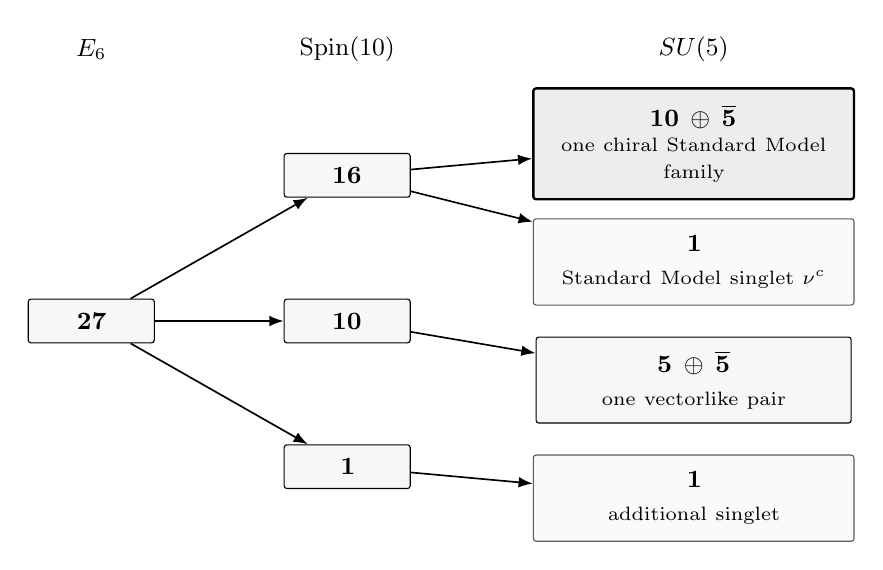
\begin{tikzpicture}[x=1cm,y=1cm]
\node[font=\small\bfseries] at (0,3.45) {$E_6$};
\node[font=\small\bfseries] at (3.25,3.45) {$\operatorname{Spin}(10)$};
\node[font=\small\bfseries] at (7.65,3.45) {$SU(5)$};

\node[repbox,text width=1.25cm] (r27) at (0,0) {$\mathbf{27}$};
\node[repbox,text width=1.25cm] (r16) at (3.25,1.85) {$\mathbf{16}$};
\node[repbox,text width=1.25cm] (r10) at (3.25,0) {$\mathbf{10}$};
\node[repbox,text width=1.25cm] (r1) at (3.25,-1.85) {$\mathbf1$};

\node[chiralbox,text width=3.65cm] (fam) at (7.65,2.25)
  {$\mathbf{10}\oplus\overline{\mathbf5}$\\[1pt]
   \scriptsize one chiral Standard Model\\[-1pt]\scriptsize family};
\node[singletbox,text width=3.65cm] (nu) at (7.65,.75)
  {$\mathbf1$\\[1pt]\scriptsize Standard Model singlet $\nu^c$};
\node[repbox,text width=3.65cm] (vec) at (7.65,-.75)
  {$\mathbf5\oplus\overline{\mathbf5}$\\[1pt]\scriptsize one vectorlike pair};
\node[singletbox,text width=3.65cm] (sg) at (7.65,-2.25)
  {$\mathbf1$\\[1pt]\scriptsize additional singlet};

\draw[branch] (r27) -- (r16);
\draw[branch] (r27) -- (r10);
\draw[branch] (r27) -- (r1);
\draw[branch] (r16) -- (fam);
\draw[branch] (r16) -- (nu);
\draw[branch] (r10) -- (vec);
\draw[branch] (r1) -- (sg);
\end{tikzpicture}
\caption{One \(\mathbf{27}\) branches into a chiral Standard Model family,
a vectorlike \(\mathbf5\oplus\overline{\mathbf5}\) pair, and two singlets.
The factor \(\mathbf{3}_M\) gives three copies of this branching.}
\label{fig:branching-27}
\end{figure}

The six singlets consist of three copies of the singlet in the
\(\mathbf{16}\) of \(\operatorname{Spin}(10)\) and three copies of the
additional singlet in the \(\mathbf{27}\) of \(E_6\).

\subsection{The faithful Standard Model group and its charge lattice}

Corollary~\ref{cor:subgroup-chain} gives one \(E_8\)-conjugacy class,
so the restriction may be computed in the block representative
\[
 \Ksm=S(U(3)\times U(2))
 \subset SU(5)\subset\operatorname{Spin}(10)\subset E_6^{\mathrm{sc}}.
\]
Its central circle has the primitive parametrisation, up to inversion,
\[
 \eta(z)=\operatorname{diag}(z^{-2}I_3,z^3I_2).
\]
This circle homomorphism is a \emph{cocharacter}; primitive means that it
traverses the circle once. Orient \(\eta\) so that the
\((\mathbf3,\mathbf2)\) in the \(\mathbf{10}\) has integer charge \(q=1\).
The conventional hypercharge used above is then \(Y=q/6\).
Let \(t\in\mathbb Z/3\) be colour triality and \(s\in\mathbb Z/2\)
weak-centre parity: the central elements
\(e^{2\pi i/3}I_3\in SU(3)\) and \(-I_2\in SU(2)\) act as
\(e^{2\pi it/3}\) and \((-1)^s\), respectively. The kernel in
Corollary~\ref{cor:subgroup-chain} says that a representation of integer
charge \(q\) descends to \(\Ksm\) exactly when
\[
 q+2t+3s\equiv0\pmod6.
\]
This congruence is the \(\mathbb Z_6\) charge lattice. When \(t=0\), it
links \(q\) to the \(SU(2)\) centre parity and forces every electric charge
in a colour-singlet multiplet to be integral.

\subsection{The net chiral index is three}

Net chirality records the difference between the multiplicities of an
irreducible representation and its dual. A dual pair contributes zero,
as does a self-dual summand. The following quotient records all these
differences at once.

Let \(R(\Ksm)\) be the additive Grothendieck group of finite-dimensional
complex representations. Let \(\chi\) be the quotient map obtained by
imposing
\(\chi(R^*)=-\chi(R)\) and \(\chi(S)=0\) for every self-dual~\(S\).
The map \(\chi\) records, for each non-self-dual pair
\(\{R,R^*\}\), the multiplicity difference \(m_R-m_{R^*}\). Applying
it to (9) gives
\[
\begin{aligned}
 \chi\!\left(V|_{\Ksm}\right)
 &=3\chi(\mathcal F_{\mathrm{SM}})
   +3\bigl(\chi(\mathbf5|_{\Ksm})
           +\chi(\overline{\mathbf5}|_{\Ksm})\bigr)
   +6\chi(\mathbf1)\\
 &=\boxed{3\chi(\mathcal F_{\mathrm{SM}})}.
\end{aligned}                                                     \tag{10}
\]
The vectorlike pairs and singlets make no contribution. Equation (10)
records net chirality; equation (9) records the full module. Duality gives
\[
 \left\{\chi\!\left(V|_{\Ksm}\right),
 \chi\!\left(V^*|_{\Ksm}\right)\right\}
 =\left\{3\chi(\mathcal F_{\mathrm{SM}}),
          -3\chi(\mathcal F_{\mathrm{SM}})\right\}.
\]
Relative to \(\chi(\mathcal F_{\mathrm{SM}})\), the coefficients \(+3\) and
\(-3\) are the chiral indices of \(V\) and \(V^*\), respectively.

\begin{corollary}[Chiral content of the classified module]
\label{cor:chiral-content}
The two orientations have chiral-index coefficients \(+3\) and \(-3\),
relative to \(\chi(\mathcal F_{\mathrm{SM}})\). Beyond this family class, no
additional net chiral class occurs in \(V\) or \(V^*\); every remaining
summand is vectorlike or a singlet.
\end{corollary}


\subsection{Local anomalies and the \texorpdfstring{\(SU(3)_M^3\)}{SU(3)M cubed} background anomaly}

\emph{Standard Model insertions.} Perturbative local cubic and linear anomaly coefficients are additive, odd
under duality, and zero on self-dual modules, so they factor through \(\chi\).
The linear coefficient governs the mixed gauge--gravitational anomaly. Since
\(\operatorname{Lie}(\Ksm)\subset\e_6=\Rad(c_V)\), the cubic anomaly of
\(V|_{\Ksm}\) vanishes. The algebra \(\e_6\) is perfect, so every
finite-dimensional trace functional on it also vanishes. Equation (10) then
shows that one copy of \(\mathcal F_{\mathrm{SM}}\), and hence three copies,
is free of perturbative gauge and mixed gauge--gravitational anomalies.

The preceding argument covers perturbative local anomalies. The spectrum in
(9) also has no mod-two \(SU(2)\) anomaly: counting colour multiplicity, each
\(\mathcal F_{\mathrm{SM}}\) contains four doublets, while each vectorlike
\(\mathbf5\oplus\overline{\mathbf5}\) contributes two. The same spectrum is
the restriction of anomaly-free \(SU(5)\) representations. For theories on spin manifolds, the bordism analysis
of the four connected Standard Model global forms gives no further global
gauge anomaly for the \(\mathbb Z_6\) quotient used here \cite{DavighiGripaiosLohitsiri}.

\medskip
\noindent\emph{The family background.} To identify the remaining cubic anomaly, let \(F_{\mathrm{SM}}\) be a
\(\Ksm\)-gauge field strength and \(F_M\) a background field strength for
\(SU(3)_M\). On
\(V=\mathbf{27}\otimes\mathbf3_M\), put
\[
F=F_{\mathrm{SM}}\otimes1_{\mathbf3}
  +1_{\mathbf{27}}\otimes F_M.
\]
The radical condition kills every cubic term containing \(F_{\mathrm{SM}}\),
and both simple factors act tracelessly. Therefore
\[
\Tr_V(F^3)=27\,\Tr_{\mathbf3}(F_M^3),
\qquad \Tr_V(F)=0. \tag{11}
\]
Every perturbative local anomaly coefficient with a \(\Ksm\) gauge insertion
vanishes, including coefficients mixed with the background \(SU(3)_M\)
field. The only remaining cubic component is the
\(SU(3)_M^3\) term, with coefficient \(27\) when \(A(\mathbf3)=1\).
As a background global symmetry, the commuting \(SU(3)_M\) carries this
perturbative \(SU(3)_M^3\) anomaly.
Promoting it to a gauge factor requires additional anomaly-cancelling structure.


\section{Conclusion}

The classification starts with an effective inclusion of compact Lie
algebras and its adjoint complement. Complex type and a nonzero cubic
radical determine the pair. Up to isomorphism of Lie-algebra pairs and
duality, the unique solution is
\[
 \mathfrak e_8\supset\mathfrak e_6\oplus\mathfrak{su}(3)_M,
 \qquad V=\mathbf{27}\boxtimes\mathbf3,
 \qquad\operatorname{Rad}(c_V)=\mathfrak e_6.
\]
Every inequivalent pair satisfying the standing algebraic hypotheses and
\(\operatorname{End}_{\mathfrak h}(\mathfrak q)\cong\mathbb C\) has zero
cubic radical. Thus no nonzero ideal \(\mathfrak k\) satisfies
\(c_V(\mathfrak k,\mathfrak h,\mathfrak h)=0\). This obstruction depends
only on the embedding and its quotient module.

The classification covers effective proper inclusions of compact real Lie
algebras of arbitrary rank. Neither algebra type, representation dimension, nor multiplicity is
prescribed. Irreducibility of \(\mathfrak q\), simplicity of \(\mathfrak g\),
and semisimplicity and maximality of \(\mathfrak h\) follow from the conditions.
They also give a compact homogeneous realization with closed subgroup;
homogeneity expresses the geometry of the pair rather than an extra
selection rule.
The finite searches arise from proved reductions and bounds; the classical
lower-rank exclusion is uniform in rank. Higher rank supplies no alternative.

Unlike a construction around a chosen group or coset, this theorem varies
the embedding and its canonical representation together. This also
distinguishes it from classifications of semisimple extensions of a supplied
gauge algebra and spectrum \cite{GomesRuhdorferToobySmith}, and from studies
of how often anomaly-free spectra admit unification \cite{HermsRuhdorfer}.
The familiar exceptional pair is characterized, not assumed.

Inside its \(E_6\) factor, the second classification gives six Weyl orbits
of maximal-subsystem triples, exactly two with a common \(A_2\) component.
In every triple, the unique largest pairwise derived group is obtained
from the \(D_5\)--\((A_5+A_1)\) pair. Using that group in the
pair-first construction gives the Standard Model and left--right chains
on the two extremal orbits, with their faithful global forms and hypercharge
embedding. The chiral dimensions \(15\) and \(16\) follow from restriction
to the intermediate groups. The full branching \textup{(9)} and chiral
class \textup{(10)} distinguish three minimal families from the additional
vectorlike pairs and singlets.

Ordinary matter is built from electrons and the lightest quarks. Their
heavier relatives carry the same gauge charges, repeating the family
pattern three times. The classified module contains that same threefold
chiral family class. Here the coefficient and the cubic-anomaly-safe ideal
are not chosen independently: they follow from one embedding.

\section*{Computational material}

The repository linked on the title page contains the exact programs,
certificates and master verification notebook \cite{ComputationalCompanion}.
The finite algorithms and completeness arguments used by the proof are
stated in Sections~3--4; the notebook supplies the reproducible calculations
and output tables.

The repository also contains Lean checks of the finite exceptional grading
calculation, the Cartan cubic test, and the stated \(E_6\) incidence
propositions. These checks use \texttt{native\_decide} with the compiler
trust described in the repository. The manuscript supplies the compact-Lie
reductions, the classical all-rank argument and the representation-theoretic
proofs around these finite checks.

\par\medskip
\noindent\textbf{AI assistance disclosure.}
This paper was created with the aid of the Intelligent Internet Zenith
system. The paper was checked with GPT-6 Astra Pro and Fable 5.1 Max.
The repository and computational verification were generated by GPT-6 Astra.

\clearpage
\begin{multicols}{2}
\begin{thebibliography}{99}
\footnotesize
\setlength{\itemsep}{0pt}
\setlength{\parsep}{0pt}
\bibitem{ParticleDataGroup}
S.~Navas et al. (Particle Data Group),
\emph{Review of Particle Physics},
Phys. Rev. D \textbf{110} (2024), 030001; 2025 update.
\bibitem{ForgacsManton}
P.~Forg\'acs and N.~S. Manton,
\emph{Space-time symmetries in gauge theories},
Commun. Math. Phys. \textbf{72} (1980), 15--35.
\bibitem{MantonFermions}
N.~S. Manton,
\emph{Fermions and parity violation in dimensional reduction schemes},
Nucl. Phys. B \textbf{193} (1981), 502--516.
\bibitem{ChaplineSlansky}
G.~Chapline and R.~Slansky,
\emph{Dimensional reduction and flavor chirality},
Nucl. Phys. B \textbf{209} (1982), 461--483.
\bibitem{ChaplineGrossman}
G.~Chapline and B.~Grossman,
\emph{Dimensional reduction example with three families of low mass fermions},
Phys. Lett. B \textbf{143} (1984), 161--164;
\textbf{144} (1984), 231--234.
\bibitem{DouzasEtAl}
G.~Douzas, T.~Grammatikopoulos, J.~Madore, and G.~Zoupanos,
\emph{Coset space dimensional reduction and classification of semi-realistic
particle physics models},
Fortschr. Phys. \textbf{56} (2008), 424--429.
\bibitem{KugoYanagida}
T.~Kugo and T.~Yanagida,
\emph{Unification of families based on a coset space
\(E_7/[SU(5)\times SU(3)\times U(1)]\)},
Phys. Lett. B \textbf{134} (1984), 313--317.
\bibitem{ItohKugoKunitomo}
K.~Itoh, T.~Kugo, and H.~Kunitomo,
\emph{Supersymmetric non-linear Lagrangians of K\"ahlerian coset spaces
\(G/H\): \(G=E_6,E_7\) and \(E_8\)},
Prog. Theor. Phys. \textbf{75} (1986), 386--426.
\bibitem{CandelasHorowitzStromingerWitten}
P.~Candelas, G.~T. Horowitz, A.~Strominger, and E.~Witten,
\emph{Vacuum configurations for superstrings},
Nucl. Phys. B \textbf{258} (1985), 46--74.
\bibitem{AlvarezGaumeGinsparg}
L.~Alvarez-Gaum\'e and P.~H. Ginsparg,
\emph{The structure of gauge and gravitational anomalies},
Ann. Phys. \textbf{161} (1985), 423--490;
erratum, Ann. Phys. \textbf{171} (1986), 233.
\bibitem{BouchiatIliopoulosMeyer}
C.~Bouchiat, J.~Iliopoulos, and P.~Meyer,
\emph{An anomaly-free version of Weinberg's model},
Phys. Lett. B \textbf{38} (1972), 519--523.
\bibitem{GrossJackiw}
D.~J. Gross and R.~Jackiw,
\emph{Effect of anomalies on quasirenormalizable theories},
Phys. Rev. D \textbf{6} (1972), 477--493.
\bibitem{Bourbaki}
N.~Bourbaki,
\emph{Lie Groups and Lie Algebras, Chapters 4--6},
Elements of Mathematics, Springer, 2002.
\bibitem{Slansky}
R.~Slansky, \emph{Group theory for unified model building},
Phys. Rep. \textbf{79} (1981), 1--128.
\bibitem{McKayPatera}
W.~G. McKay and J.~Patera,
\emph{Tables of Dimensions, Indices, and Branching Rules for
Representations of Simple Lie Algebras},
Lecture Notes in Pure and Applied Mathematics, vol.~69,
Marcel Dekker, New York, 1981.
\bibitem{BarsGunaydin}
I.~Bars and M.~G\"unaydin,
\emph{Grand unification with the exceptional group \(E_8\)},
Phys. Rev. Lett. \textbf{45} (1980), 859--862.
\bibitem{OrbifoldIntersections}
W.~Buchm\"uller, K.~Hamaguchi, O.~Lebedev, and M.~Ratz,
\emph{Dual models of gauge unification in various dimensions},
Nucl. Phys. B \textbf{712} (2005), 139--156.
\bibitem{PatiSalam}
J.~C. Pati and A.~Salam,
\emph{Lepton number as the fourth color},
Phys. Rev. D \textbf{10} (1974), 275--289;
erratum, Phys. Rev. D \textbf{11} (1975), 703.
\bibitem{GeorgiGlashow}
H.~Georgi and S.~L. Glashow,
\emph{Unity of all elementary-particle forces},
Phys. Rev. Lett. \textbf{32} (1974), 438--441.
\bibitem{FritzschMinkowski}
H.~Fritzsch and P.~Minkowski,
\emph{Unified interactions of leptons and hadrons},
Ann. Phys. \textbf{93} (1975), 193--266.
\bibitem{GurseyRamondSikivie}
F.~G\"ursey, P.~Ramond, and P.~Sikivie,
\emph{A universal gauge theory model based on \(E_6\)},
Phys. Lett. B \textbf{60} (1976), 177--180.
\bibitem{BaezHuerta}
J.~C. Baez and J.~Huerta,
\emph{The algebra of grand unified theories},
Bull. Amer. Math. Soc. \textbf{47} (2010), 483--552.
\bibitem{Krasnov}
K.~Krasnov,
\emph{Geometry of \(\operatorname{Spin}(10)\) symmetry breaking},
J. Math. Phys. \textbf{65} (2024), 082302.
\bibitem{TodorovDuboisViolette}
I.~Todorov and M.~Dubois-Violette,
\emph{Deducing the symmetry of the Standard Model from the automorphism and
structure groups of the exceptional Jordan algebra},
Int. J. Mod. Phys. A \textbf{33} (2018), 1850118.
\bibitem{SugenoWada}
T.~Sugeno and H.~Wada,
\emph{Anomalies in family unification models from bordism classification},
arXiv:2604.04393 [hep-th] (2026).
\bibitem{DavighiGripaiosLohitsiri}
J.~Davighi, B.~Gripaios, and N.~Lohitsiri,
\emph{Global anomalies in the Standard Model(s) and beyond},
JHEP \textbf{07} (2020), 232.
\bibitem{GomesRuhdorferToobySmith}
A.~Gomes, M.~Ruhdorfer, and J.~Tooby-Smith,
\emph{Semisimple unifications of any gauge theory},
Phys. Rev. D \textbf{108} (2023), 075001;
arXiv:2306.16439 [hep-ph].
\bibitem{HermsRuhdorfer}
J.~Herms and M.~Ruhdorfer,
\emph{How common are grand unified theories?},
Phys. Rev. D \textbf{112} (2025), 115041;
arXiv:2408.11089 [hep-ph].
\bibitem{ComputationalCompanion}
E.~Mostaque,
\emph{Computational companion to From Chirality to the Standard Model},
source code and exact certificates (2026).
\url{https://github.com/emad-ii/chirality-standard-model}.
\end{thebibliography}
\end{multicols}

\end{document}
